\exercisesection{1}

\begin{enumerate}
\def\labelenumi{\arabic{enumi}.}
\tightlist
\item
  \begin{enumerate}
  \def\labelenumii{(\alph{enumii})}
  \tightlist
  \item
    Let A be an absolutely flat ring (Chapter I, §2, Exercise 17). Show that Ass(A) is the set of isolated points of Spec(A) (note that Ass(A) is the set of prime ideals which are annihilators of an idempotent of A).
  \end{enumerate}
\end{enumerate}

\begin{enumerate}
\def\labelenumi{(\alph{enumi})}
\setcounter{enumi}{1}
\item
  Deduce from (a) an example of a ring A such that \(A \neq 0\) and \(\operatorname{Ass}(A) = \varnothing\) (cf.~Chapter II, §4, Exercise 17) and for which the conclusion of no. 1, Corollary 2 to Proposition 2 does not hold.
\item
  Deduce from (b) an example of a ring A and a multiplicative subset S of A such that the mapping \(p \mapsto S^{-1}p\) of \(\text{Ass}(A) \cap \Phi\) to \(\text{Ass}(S^{-1}A)\) (no. 2, Proposition 5) is not surjective.
\end{enumerate}

* 2. Let K be a commutative field and A the valuation ring, whose order group is Q, consisting of the ``formal power series'' \(\sum_{r} c_r T^r\) , where \(c_r \in K\) , \(r \in \mathbf{Q}_+\) and the set of \(r\) such that \(c_r \neq 0\) is well ordered. Let \(\alpha\) be an irrational number \(>0\) , \(a\) the ideal of A consisting of the elements with valuation \(>\alpha\) and C the ring A/a. Then \(\text{Spec(C)}\) reduces to a point \(p\) ; for all \(x \neq 0\) in C, \(px \neq 0\) , but for all \(\lambda \in p\) , there exists \(y \neq 0\) in C such that \(\lambda y = 0\) . In particular, \(\text{Ass(C)} = \varnothing\) , although \(\text{Supp(C)} = \text{Spec(C)} = \{\mathfrak{p}\}\) . *

\begin{enumerate}
\def\labelenumi{\arabic{enumi}.}
\setcounter{enumi}{2}
\item
  Let M be an A-module and N a submodule of M. Show that every prime ideal \(\mathfrak{p} \in \operatorname{Ass}(M/N)\) which does not contain Ann(N) is associated with M. Give an example of an ideal p belonging to Ass(M/N) but not to Ass(M) (take A to be an integral domain, M = A).
\item
  Give an example of a ring A such that M = A does not satisfy the conclusion of Theorem 1 of no. 4 (cf.~Exercise 1 (b)).
\item
  Let A = K{[}X, Y{]} be the polynomial algebra in two indeterminates over a commutative field K and a the maximal ideal AX + AY of A. Show that \(\text{Supp}(a) = \text{Spec}(A)\) is infinite and \(\text{Ass}(a) = \{0\}\) . Prove that there is no composition series of a all of whose factor modules are isomorphic to A. (The existence of such a series would imply that a was isomorphic to a module \(A^{n}\) ; then necessarily n = 1, which is absurd.)
\end{enumerate}

¶ 6. Let A be a ring and E an A-module.

\begin{enumerate}
\def\labelenumi{(\alph{enumi})}
\item
  Show that for a prime ideal p of A to belong to Supp(E), it is necessary and sufficient that there exist a submodule F of E such that \(p \in \text{Ass}(E/F)\) (to see that the condition is necessary, consider a submodule F of E of the form px, where \(x \in E\) ; to see that the condition is sufficient, use Proposition 7 of no. 3).
\item
  Suppose that A is Noetherian and E finitely generated. Show that for every prime ideal \(\mathfrak{p}\in\operatorname{Supp}(\mathrm{E})\) , there exists a composition series \((\mathrm{E}_{i})_{0\leqslant i\leqslant n}\) of E such that, for \(0\leqslant i\leqslant n-1\) , \(E_{i}/E_{i+1}\) is isomorphic to \(A/p_{i}\) , where \(p_{i}\) is a prime ideal and one of the \(p_{i}\) is equal to p.
\end{enumerate}

\begin{enumerate}
\def\labelenumi{\arabic{enumi}.}
\setcounter{enumi}{6}
\tightlist
\item
  Let A be a Noetherian ring, M a finitely generated A-module and \(\mathfrak{a} = \text{Ann}(M)\) .
\end{enumerate}

\begin{enumerate}
\def\labelenumi{(\alph{enumi})}
\item
  Show that, if \(\mathfrak{a}\) is prime, \(\mathfrak{a}\) is the least element of \(\operatorname{Ass}(\mathbf{M})\) . (Note that \(\mathfrak{a} = \bigcap_{\mathfrak{p} \in \operatorname{Ass}(\mathbf{M})} \mathfrak{p}\) .)
\item
  Show that every prime ideal associated with A/a is associated with M. (Note that if p is a prime ideal of A the annihilator of the class in A/a of an element \(\alpha \in A\) , then \(\mathfrak{p} = \operatorname{Ann}(\alpha\mathbf{M})\) and use (a).)
\item
  Let \(p, q\) be two distinct prime ideals of \(A\) such that \(p \subset q\) . Show that, if \(M = (A/p) \oplus (A/q)\) , then \(\operatorname{Ass}(A/a) \neq \operatorname{Ass}(M)\) .
\end{enumerate}

\begin{enumerate}
\def\labelenumi{\arabic{enumi}.}
\setcounter{enumi}{7}
\item
  Let A be a Noetherian ring, a an ideal of A, M a finitely generated A-module and P the submodule of M consisting of the \(x \in M\) such that ax = 0. Show that \(\operatorname{Ass}(M/P) \subset \operatorname{Ass}(M)\) (note that for all \(x \in M\) the annihilator of \((Ax + P)/P\) is also that of ax and use Exercise 7 (a)).
\item
  Let A be a Noetherian ring and a an ideal of A.
\end{enumerate}

\begin{enumerate}
\def\labelenumi{(\alph{enumi})}
\item
  For an ideal b of A to satisfy a: b ≠ a, it is necessary and sufficient that b be contained in a prime ideal p ∈ Ass(A/a).
\item
  Let A be the polynomial algebra K{[}X, Y, Z{]} in 3 indeterminates over a field K. Let n = AX, m = AX + AY + AZ, a = n ∩ m². Show that there is a prime ideal p containing a such that a: p ≠ a but which is not a prime ideal associated with A.
\end{enumerate}

\begin{enumerate}
\def\labelenumi{\arabic{enumi}.}
\setcounter{enumi}{9}
\tightlist
\item
  \begin{enumerate}
  \def\labelenumii{(\alph{enumii})}
  \tightlist
  \item
    Give an example of a Z-module M such that \(\operatorname{Ass}(\operatorname{Hom}_{\mathbf{Z}}(\mathbf{M}, \mathbf{M}))\) is not contained in \(\operatorname{Supp}(\mathbf{M})\) (cf.~Chapter II, § 4, Exercise 24 (c)).
  \end{enumerate}
\end{enumerate}

\begin{enumerate}
\def\labelenumi{(\alph{enumi})}
\setcounter{enumi}{1}
\tightlist
\item
  Give an example of Z-modules E, F such that
\end{enumerate}

\[
\operatorname{Ass} \left(\operatorname{Hom} _ {\mathbf {Z}} (\mathrm{E}, \mathrm{F})\right) = \varnothing ,
\]

but \(\operatorname{Ass}(\mathbf{F}) \cap \operatorname{Supp}(\mathbf{E}) \neq \varnothing\) (take \(\mathbf{F} = \mathbf{Z}\) ).

\begin{enumerate}
\def\labelenumi{\arabic{enumi}.}
\setcounter{enumi}{10}
\tightlist
\item
  \begin{enumerate}
  \def\labelenumii{(\alph{enumii})}
  \tightlist
  \item
    Let \(\mathbf{A}\) be a Noetherian ring and \(\mathbf{E}\) an \(\mathbf{A}\) -module. Show that the canonical homomorphism of E to the product \(\prod_{p\in\text{Ass}(E)}E_p\) is injective (if N is the kernel of this homomorphism, show that \(\text{Ass}(N)=\varnothing\) ).
  \end{enumerate}
\end{enumerate}

\begin{enumerate}
\def\labelenumi{(\alph{enumi})}
\setcounter{enumi}{1}
\tightlist
\item
  Take A to be the polynomial ring K{[}X,Y,Z{]} over a field K; let \(p_{1}=AX+AY\) , \(p_{2}=AX+AZ\) , which are prime ideals and a the ideal \(p_{1}p_{2}\) . The set \(\operatorname{Ass}(A/a)\) consists of \(p_{1}\) , \(p_{2}\) and the maximal ideal \(m=p_{1}+p_{2}\) ; show that the canonical homomorphism from E=A/a to \(E_{p_{1}}\times E_{p_{2}}\) is not injective.
\end{enumerate}

\begin{enumerate}
\def\labelenumi{\arabic{enumi}.}
\setcounter{enumi}{11}
\tightlist
\item
  Let A be a Noetherian ring and P a projective A-module. Show that, if, for all \(p \in \text{Ass}(A)\) , \(P_{p}\) is a finitely generated \(A_{p}\) -module, then P is a finitely generated A-module (embed A in the product \(\prod_{p \in \text{Ass}(A)} A_{p}\) (Exercise 11) and use Algebra, Chapter II, § 5, no. 5, Proposition 9).
\end{enumerate}

¶ 13. Let A be a Noetherian ring, E a finitely generated A-module, p, q two prime ideals of A such that \(p \subset q\) and a an element of q. Suppose that \(p \in \text{Ass}(E)\) and that the homothety \(a_{E}\) is injective. Show that there exists a prime ideal \(n \in \text{Ass}(E/aE)\) such that \(p + Aa \subset n \subset q\) . (Replacing A by \(A_{q}\) , we may assume that A is local with maximal ideal q. Let \(F \neq 0\) be the submodule of E consisting of the x such that px = 0. Show that the relation \(F \subset aE\) would imply F = aF and obtain a contradiction using Nakayama's Lemma. Then use Proposition 8 of no. 4.)

\begin{enumerate}
\def\labelenumi{\arabic{enumi}.}
\setcounter{enumi}{13}
\item
  Let A be an integral domain, \(a \neq 0\) an element of A and p an element of \(\operatorname{Ass}(A/aA)\) . Show that, for every element \(b \neq 0\) of p, \(\mathfrak{p} \in \operatorname{Ass}(A/bA)\) (if \(c \in A\) is such that the relation \(xc \in aA\) is equivalent to \(x \in p\) , show that there exists \(d \in A\) such that \(xd \in bA\) is equivalent to \(xc \in aA\) ).
\item
  Let A be a Noetherian ring, E a finitely generated A-module, F a submodule of E and m an ideal of A. For F to be closed in E under the m-adic topology, it is necessary and sufficient that \(p + m \neq A\) for every ideal \(p \in \text{Ass}(E/F)\) . (Reduce it to the case where F = 0, use Chapter III, §3, no. 2, Corollary to Proposition 5 and apply Corollary 2 to Proposition 2 of no. 1 to an element \(1 + m\) , where \(m \in m\) .)
\item
  Let A be a Noetherian ring. For A to be isomorphic to a finite product of integral domains, it is necessary and sufficient that for every prime ideal p of A the local ring \(A_{p}\) be an integral domain. (To see that the condition is sufficient, note first that it implies that that ring A is reduced; deduce that \(\{0\} = \bigcap_{i} p_{i}\) , where the \(p_{i} (1 \leqslant i \leqslant n)\) are the minimal prime ideals of A. Show that, for \(i \neq j\) , of necessity \(p_{i} + p_{j} = A\) ; for this, note that, if there existed a maximal ideal m containing \(p_{i} + p_{j}\) , the ring \(A_{m}\) would not be an integral domain, using Corollary 3 to Proposition 2 of no. 1, and the Corollary to Proposition 5 of no. 2.)
\end{enumerate}

¶ 17. Let A be a ring and M an A-module. A prime ideal p of A is said to be weakly associated with M if there exists \(x \in \mathbf{M}\) such that p is a minimal element of the set of prime ideals containing Ann(x); we denote by \(\operatorname{Ass}_{f}(\mathbf{M})\) the set of ideals weakly associated with M. Then \(\operatorname{Ass}(\mathbf{M}) \subset \operatorname{Ass}_{f}(\mathbf{M})\) .

\begin{enumerate}
\def\labelenumi{(\alph{enumi})}
\item
  Show that the relation \(\mathbf{M} \neq 0\) is equivalent to \(\operatorname{Ass}_f(\mathbf{M}) \neq \varnothing\) .
\item
  For \(a \in \mathbf{A}\) to be such that \(a_{\mathbf{M}}\) is injective, it is necessary and sufficient that \(a\) belong to no element of \(\operatorname{Ass}_f(\mathbf{M})\) (note that, if \(a\) belongs to the radical of an ideal \(\operatorname{Ann}(x)\) where \(x \neq 0\) in \(\mathbf{M}\) , there exists \(y \neq 0\) in \(\mathbf{M}\) such that \(a \in \operatorname{Ann}(y)\) . To show that the condition is necessary, reduce it, by considering the ring \(\operatorname{A}/\operatorname{Ann}(x)\) , to proving that in a ring \(\mathbf{A}\) every element belonging to a prime ideal \(p\) which is minimal in the set of prime ideals of \(\mathbf{A}\) is necessarily a divisor of 0 (Chapter II, § 2, no. 6, Proposition 12).)
\end{enumerate}

For \(a \in A\) to be such that \(a_{M}\) is almost nilpotent, it is necessary and sufficient that a belongs to all the elements of \(\operatorname{Ass}_{f}(M)\) .

\begin{enumerate}
\def\labelenumi{(\alph{enumi})}
\setcounter{enumi}{2}
\tightlist
\item
  If \(\mathbf{N}\) is a submodule of \(\mathbf{M}\) , then
\end{enumerate}

\[
\operatorname{Ass} _ {f} (\mathbf {N}) \subset \operatorname{Ass} _ {f} (\mathbf {M}) \subset \operatorname{Ass} _ {f} (\mathbf {N}) \cup \operatorname{Ass} _ {f} (\mathbf {M} / \mathbf {N}).
\]

(Note that, if \(\mathfrak{p}\) is a prime ideal, \(a \notin \mathfrak{p}\) , \(x \in \mathbf{M}\) such that \(ax \in \mathbf{N}\) and \(\operatorname{Ann}(x) \subset \mathfrak{p}\) , then \(\operatorname{Ann}(ax) \subset \mathfrak{p}\) .)

\begin{enumerate}
\def\labelenumi{(\alph{enumi})}
\setcounter{enumi}{3}
\item
  Let S be a multiplicative subset of A and \(\Phi\) the set of prime ideals of A not meeting S. Show that \(p \mapsto S^{-1}p\) is a bijection of \(\operatorname{Ass}_{f}(M) \cap \Phi\) onto \(\operatorname{Ass}_{f}(S^{-1}M)\) . (Observe that the inverse image under the canonical mapping \(A \to S^{-1}A\) of the annihilator of an element x/s, where \(x \in M\) , \(s \in S\) , is the saturation with respect to S of \(\operatorname{Ann}(x)\) .)
\item
  Let S be a multiplicative subset of A; show that, if N is the kernel of the canonical homomorphism \(M \to S^{-1}M\) , \(\operatorname{Ass}_{f}(N)\) is the set of \(p \in \operatorname{Ass}_{f}(M)\) which meet S and \(\operatorname{Ass}_{f}(M/N)\) the set of \(p \in \operatorname{Ass}_{f}(M)\) which do not meet S. (To prove the latter point, consider a prime ideal q which is minimal in the set of those containing \(\operatorname{Ann}(\bar{y})\) , where \(\bar{y} \in M/N\) ; note that, if \(y \in \bar{y}\) and \(t \in q\) , there exists \(c \notin q\) and an integer n \textgreater{} 0 such that \(ct^{n}y \in N\) (Chapter II, §2, no. 6, Proposition 12); deduce first that \(q \cap S = \varnothing\) . There exists \(s \in S\) such that \(sct^{n}y = 0\) ; conclude that there can be no prime ideal \(q' \neq q\) such that \(\operatorname{Ann}(y) \subset q' \subset q\) .)
\item
  For a prime ideal of \(\mathbf{A}\) to belong to \(\operatorname{Supp}(\mathbf{M})\) , it is necessary and sufficient that it contains an element of \(\operatorname{Ass}_f(\mathbf{M})\) .
\item
  Show that, if A is Noetherian, \(\operatorname{Ass}_f(M) = \operatorname{Ass}(M)\) .
\item
  If \(\mathbf{A}\) is an absolutely flat ring, then \(\operatorname{Ass}_f(\mathbf{A}) = \operatorname{Spec}(\mathbf{A})\) .
\item
  For every A-module E the canonical homomorphism from E to the product
\end{enumerate}

\(\prod_{p\in\mathrm{Ass}_{f}(\mathbf{E})}\mathrm{E}_{p}\) is injective; in other words, the intersection of the saturations of \(\{0\}\) in E with respect to the ideals \(p\in\mathrm{Ass}_{f}(\mathbf{E})\) is reduced to 0. Generalize Exercise 12 similarly.

\begin{enumerate}
\def\labelenumi{(\alph{enumi})}
\setcounter{enumi}{9}
\tightlist
\item
  Let M be a finitely generated A-module. Show that the minimal elements of the set of prime ideals containing \(\mathfrak{a} = \text{Ann}(M)\) belong to \(\text{Ass}_{f}(M)\) (if \((x_{i})_{1 \leq i \leq n}\) is a system of generators of M, show that such an ideal contains one of the \(\text{Ann}(x_{i})\) ). Deduce that \(\text{Ass}_{f}(A/a)\) is contained in \(\text{Ass}_{f}(M)\) (if a prime ideal p contains the annihilator of the class mod. a of an element \(\alpha \in A\) , note that p contains the annihilator of the submodule \(\alpha M\) of M); show that \(\text{Ass}_{f}(A/a)\) , \(\text{Ass}(M)\) and the set of prime ideals containing a have the same minimal elements.
\end{enumerate}

\begin{enumerate}
\def\labelenumi{\arabic{enumi}.}
\setcounter{enumi}{17}
\tightlist
\item
  Let A be a ring and M an A-module. For an element \(c \in A\) to be such that, for all \(a \in A\) such that the homothety \(a_{M}\) is injective, \(b_{M}\) is an injective homothety for all b of the form \(a + \lambda c\) , where \(\lambda \in A\) , it is sufficient that c belong to the intersection of the maximal elements of \(\operatorname{Ass}_{f}(M)\) (use Exercise 17 (b)). Is this condition necessary?
\end{enumerate}

* 19. Let A be the ring of a valuation of height 2, \(\Gamma\) its order group, \(\Gamma_1\) the unique isolated subgroup of \(\Gamma\) distinct from \(\{0\}\) and \(\Gamma\) and \(\gamma > 0\) an element of \(\Gamma\) not belonging to \(\Gamma_1\) . Let \(a\) be the ideal of those \(x \in A\) such that \(v(x) \geqslant \gamma\) , \(b\) the ideal of those \(x \in A\) such that \(v(x) > \gamma\) , \(E = A/a\) and \(F = A/b\) . Show that \(\operatorname{Ass}_f(\operatorname{Hom}_A(E, F))\) is distinct from \(\operatorname{Ass}_f(F) \cap \operatorname{Supp}(E)\) . *

\exercisesection{2}

\begin{enumerate}
\def\labelenumi{\arabic{enumi}.}
\tightlist
\item
  \begin{enumerate}
  \def\labelenumii{(\alph{enumii})}
  \tightlist
  \item
    Show that in the Noetherian polynomial ring \(\mathbf{A} = \mathbf{Z}[\mathbf{X}]\) in one indeterminate over \(\mathbf{Z}\) , the ideal \(m = 2A + AX\) is maximal and that the ideal \(q = 4A + AX\) is m-primary, but is not equal to a power of \(m\) .
  \end{enumerate}
\end{enumerate}

\begin{enumerate}
\def\labelenumi{(\alph{enumi})}
\setcounter{enumi}{1}
\item
  In the ring \(\mathbf{B} = \mathbf{Z}[2\mathbf{X},\mathbf{X}^2,\mathbf{X}^3] \subset \mathbf{A}\) which is Noetherian, show that the ideal \(\mathfrak{p} = 2\mathrm{BX} + \mathrm{BX}^2\) is prime, but that \(\mathfrak{p}^2\) is not \(\mathfrak{p}\) -primary, although its radical is equal to \(\mathfrak{p}\) .
\item
  Let \(\mathbf{K}\) be a commutative field and \(\mathbf{A}\) the quotient ring of \(\mathbf{K}[\mathbf{X},\mathbf{Y},\mathbf{Z}]\) by the ideal generated by \(Z^2 -\mathbf{XY}\) ; let \(x,y,z\) be the canonical images of \(\mathbf{X},\mathbf{Y},\mathbf{Z}\) in \(\mathbf{A}\) . Show that \(\mathfrak{p} = \mathbf{A}x + \mathbf{A}z\) is prime, that \(\mathfrak{p}^2\) is not primary and that \(\mathfrak{p}^2 = \mathfrak{a}\cap \mathfrak{b}^2\) is a primary decomposition of \(\mathfrak{p}^2\) , where \(\mathfrak{a} = \mathbf{A}x\) and \(\mathfrak{b} = \mathbf{A}x + \mathbf{A}y + \mathbf{A}z\) .
\end{enumerate}

\begin{enumerate}
\def\labelenumi{\arabic{enumi}.}
\setcounter{enumi}{1}
\item
  In the example of Exercise 11 (b) of §1, show that \(\mathfrak{a} = \mathfrak{m}^2 \cap \mathfrak{p}_1 \cap \mathfrak{p}_2\) is a reduced primary decomposition of \(\mathfrak{a}\) in \(\mathbf{A}\) and that the saturation of \(\mathfrak{a}\) with respect to \(\mathfrak{m}\) is equal to \(\mathfrak{a}\) (and is therefore not primary).
\item
  Let A be a Noetherian ring and M a finitely generated A-module. Let Q be a p-primary submodule in M. The greatest lower bound of the integers \(n \geqslant 1\) such that \(p^{n}M \subset Q\) is called the exponent of Q in M and denoted by \(e(M/Q)\) .
\end{enumerate}

Let \((Q_{\lambda})_{\lambda \in L}\) be a family of \(p\) -primary submodules in M. For \(Q = \bigcap_{\lambda \in L} Q_{\lambda}\) to be p-primary in M, it is necessary and sufficient that the family \((e(\mathbf{M}/\mathbf{Q}_{\lambda}))_{\lambda\in\mathbf{L}}\) be bounded above; then \(e(\mathbf{M}/\mathbf{Q})\geqslant e(\mathbf{M}/\mathbf{Q}_{\lambda})\) for all \(\lambda\in L\) .

¶ 4. Let A be a Noetherian ring and M a finitely generated A-module. Let p be an element of Ass(M) and let \(\mathfrak{G}_{\mathfrak{p}}\) be the set of submodules Q of M such that \(\operatorname{Ass}(M/Q) = \{\mathfrak{p}\}\) and \(\operatorname{Ass}(Q) = \operatorname{Ass}(M) - \{\mathfrak{p}\}\) (a set which is not empty by § 1, no. 1, Proposition 4). We write \(e_{\mathfrak{p}}(M) = \inf_{\mathbf{Q} \in \mathfrak{G}_{\mathfrak{p}}} e(M/Q)\) (Exercise 3).

\begin{enumerate}
\def\labelenumi{(\alph{enumi})}
\item
  Let \(n_{\mathfrak{p}}\) be an integer \(\geqslant e_{\mathfrak{p}}(\mathbf{M})\) and let \(\mathfrak{F}(n_{\mathfrak{p}})\) be the subset of \(\mathfrak{G}_{\mathfrak{p}}\) consisting of the submodules \(\mathbf{Q}\) such that \(e(\mathbf{M} / \mathbf{Q}) \leqslant n_{\mathfrak{p}}\) . Show that \(\mathfrak{F}(n_{\mathfrak{p}})\) has a least element \(\mathbf{Q}(\mathfrak{p}, n_{\mathfrak{p}})\) .
\item
  Let \((n_{\mathfrak{p}})_{\mathfrak{p} \in \operatorname{Ass}(\mathbf{M})}\) be a family of integers such that \(n_{\mathfrak{p}} \geqslant e_{\mathfrak{p}}(\mathbf{M})\) for all \(\mathfrak{p} \in \operatorname{Ass}(\mathbf{M})\) . Show that the submodules \(\mathbf{Q}(\mathfrak{p}, n_{\mathfrak{p}})\) corresponding to this family form a reduced primary decomposition of \(\{0\}\) in \(\mathbf{M}\) said to be canonically determined by the family \((n_{\mathfrak{p}})\) . If we take \(n_{\mathfrak{p}} = e_{\mathfrak{p}}(\mathbf{M})\) for all \(\mathfrak{p} \in \operatorname{Ass}(\mathbf{M})\) , the primary decomposition consisting of the \(\mathbf{Q}(\mathfrak{p}) = \mathbf{Q}(\mathfrak{p}, e_{\mathfrak{p}}(\mathbf{M}))\) is called the canonical primary decomposition of \(\{0\}\) in \(\mathbf{M}\) . Let \(\{0\} = \bigcap_{\mathfrak{p} \in \operatorname{Ass}(\mathbf{M})} \mathbf{Q}'(\mathfrak{p})\) be any reduced primary decomposition of \(\{0\}\) in \(\mathbf{M}\) . Show that \(e(\mathbf{M}/\mathbf{Q}(\mathfrak{p})) \leqslant e(\mathbf{M}/\mathbf{Q}'(\mathfrak{p}))\) for all \(\mathfrak{p} \in \operatorname{Ass}(\mathbf{M})\) and that, if \(e(\mathbf{M}/\mathbf{Q}(\mathfrak{p})) = e(\mathbf{M}/\mathbf{Q}'(\mathfrak{p}))\) for some \(\mathfrak{p}\) , then \(\mathbf{Q}(\mathfrak{p}) \subset \mathbf{Q}'(\mathfrak{p})\) (``Theorem of Ortiz'').
\item
  Show that \(\mathbf{Q}(\mathfrak{p}, n_{\mathfrak{p}})\) is the saturation of \(\mathfrak{p}^{n_{\mathfrak{p}}} \mathbf{M}\) with respect to \(\mathfrak{p}\) (use § 1, no. 2, Proposition 6); \(\mathfrak{p}\) is the least element of \(\operatorname{Supp}(\mathbf{M} / \mathfrak{p}^n\mathbf{M})\) .
\item
  Let S be a multiplicative subset of A not meeting a prime ideal \(\mathfrak{p} \in \operatorname{Ass}(M)\) and let Q be a p-primary submodule of M. Show that \(e(\mathrm{M}/\mathrm{Q}) = e(\mathrm{S}^{-1}\mathrm{M}/\mathrm{S}^{-1}\mathrm{Q})\) . Show that, if S is a multiplicative subset of A, \(\Phi\) the set of \(\mathfrak{p} \in \operatorname{Ass}(M)\) such that \(S \cap \mathfrak{p} = \varnothing\) and N the saturation of \(\{0\}\) in M with respect to S, the \(\mathrm{Q}(\mathfrak{p}, n_{\mathfrak{p}})\) where \(\mathfrak{p} \in \Phi\) form the reduced primary decomposition of N in M canonically determined by the family \((n_{\mathfrak{p}})_{\mathfrak{p} \in \Phi}\) and the \(S^{-1}\mathrm{Q}(\mathfrak{p}, n_{\mathfrak{p}})\) where \(\mathfrak{p} \in \Phi\) the reduced primary decomposition of \(\{0\}\) in \(S^{-1}M\) canonically determined by the family \((n_{\mathfrak{p}})_{\mathfrak{p} \in \Phi}\) . Consider the particular case of canonical primary decompositions.
\end{enumerate}

\begin{enumerate}
\def\labelenumi{\arabic{enumi}.}
\setcounter{enumi}{4}
\item
  Let L be a finitely generated free Z-module and T a finite commutative group whose order is a power of a prime number p.~Show that the canonical primary decomposition (Exercise 4) of \(\{0\}\) in \(M = L \oplus T\) is \(\{0\} = p^{n}L \cap T\) , where n is the least integer \(\geqslant 0\) such that \(p^{n}T = 0\) (note that \(p^{n}M = p^{n}L\) ).
\item
  In Exercise 5 of § 1, \{0\} is primary in the A-module a relative to the prime ideal \{0\} of A. Show that the submodule AX of a is primary with respect to a relative to a prime ideal \(\neq\{0\}\) and that the submodule AXY of a is not primary with respect to a.
\item
  Let \(\mathbf{A}\) be a Noetherian ring, \(\mathbf{M}\) a finitely generated A-module and \((\mathfrak{p}_i)_{1\leqslant i\leqslant n}\) a sequence obtained by arranging the elements of \(\operatorname {Ass}(\mathbf{M})\) in any order. Show that there exists a composition series \((\mathbf{M}_i)_{0\leqslant i\leqslant n}\) of \(\mathbf{M}\) such that, for \(0\leqslant i\leqslant n - 1\) , \(\mathbf{M}_{i + 1}\) is \(p_i\) primary in \(\mathbf{M}_i\) (use Proposition 4 of no. 3).
\end{enumerate}

¶ 8. Let A be a Noetherian ring, E a finitely generated A-module, F a submodule of E and m an ideal of A. Let \(\mathbf{F} = \bigcap_{\mathfrak{p} \in \operatorname{Ass}(\mathbf{E}/\mathbf{F})} \mathbf{Q}(\mathfrak{p})\) be a reduced primary decomposition of F in E. Show that the closure of F in E under the m-adic topology on E is equal to \(\bigcap_{\mathfrak{p} \in \Phi} \mathbf{Q}(\mathfrak{p})\) , where \(\Phi\) is the set of \(\mathfrak{p} \in \operatorname{Ass}(\mathbf{E}/\mathbf{F})\) such that \(\mathfrak{p} + \mathfrak{m} \neq \mathbf{A}\) . (Consider first the case where F is p-primary in E and show that, if \(\mathfrak{p} + \mathfrak{m} = \mathbf{A}\) , F is dense in E; proceed to the general case using Exercise 15 of § 1 and Chapter III, § 3, no. 4, Corollary 1 to Theorem 3).

\begin{enumerate}
\def\labelenumi{\arabic{enumi}.}
\setcounter{enumi}{8}
\item
  Let A be a Noetherian ring, m a maximal ideal of A and M an A-module such that \(\{0\}\) is m-primary in M. If \(\hat{A}\) is the Hausdorff completion of A with respect to the m-adic topology, show that the canonical mapping \(M \to M \otimes_{A} \hat{A}\) is bijective (consider first the case where M is finitely generated, using Proposition 7 of no. 5; in the general case, consider M as the direct limit of its finitely generated submodules).
\item
  Let A be a Noetherian ring and M an A-module. Show that the following properties are equivalent:
\end{enumerate}

\((\alpha)\) Every finitely generated submodule of \(\mathbf{M}\) is of finite length.

(β) M is a direct limit of A-modules of finite length.

(γ) Every element \(\mathfrak{p} \in \operatorname{Ass}(\mathbf{M})\) is a maximal ideal of A.

(δ) Every element \(\mathfrak{p} \in \operatorname{Supp}(\mathbf{M})\) is a maximal ideal of A.

\begin{enumerate}
\def\labelenumi{\arabic{enumi}.}
\setcounter{enumi}{10}
\tightlist
\item
  Let A be a ring, M an A-module and N a submodule of M. The set of \(a \in A\) such that the homothety of ratio a on M/N is almost nilpotent is called the radical of N in M and denoted by \(\mathfrak{r}_{\mathrm{M}}(\mathrm{N})\) . Show that \(\mathfrak{r}_{\mathrm{M}}(\mathrm{N})\) is an ideal of A and that, for all \(p \in \operatorname{Ass}_{f}(\mathrm{M}/\mathrm{N})\) , \(\mathfrak{r}_{\mathrm{M}}(\mathrm{N}) \subset p\) . If \(N_{1}, N_{2}\) are two submodules of M, then \(\mathfrak{r}_{\mathrm{M}}(\mathrm{N}_{1} \cap \mathrm{N}_{2}) = \mathfrak{r}_{\mathrm{M}}(\mathrm{N}_{1}) \cap \mathfrak{r}_{\mathrm{M}}(\mathrm{N}_{2})\) ; if a is an ideal of A, \(\mathfrak{r}_{\mathrm{M}}(\mathfrak{a}\mathrm{N}) \supset \mathfrak{r}(\mathfrak{a}) \cap \mathfrak{r}_{\mathrm{M}}(\mathrm{N})\) and \(\mathfrak{r}_{\mathrm{A}}(\mathfrak{a}) = \mathfrak{r}(\mathfrak{a})\) .
\end{enumerate}

¶ 12. Let A be a ring, M an A-module and N a submodule of M.

\begin{enumerate}
\def\labelenumi{(\alph{enumi})}
\item
  For \(\operatorname{Ass}_f(\mathbf{M} / \mathbf{N})\) (§ 1, Exercise 17) to be reduced to a single element \(\mathfrak{p}\) , it is necessary and sufficient that \(\mathbf{N} \neq \mathbf{M}\) and that, for all \(a \in \mathbf{A}\) , the homothety with ratio \(a\) on \(\mathbf{M} / \mathbf{N}\) be injective or almost nilpotent; then \(\mathfrak{p} = \mathfrak{r}_{\mathbf{M}}(\mathbf{N})\) (Exercise 11) and we also say that \(\mathbf{N}\) is primary (or \(\mathfrak{p}\) -primary) in \(\mathbf{M}\) . For every submodule \(\mathbf{M}'\) of \(\mathbf{M}\) such that \(\mathbf{N} \subset \mathbf{M}'\) and \(\mathbf{N} \neq \mathbf{M}'\) , \(\mathbf{N}\) is then \(\mathfrak{p}\) -primary in \(\mathbf{M}'\) .
\item
  If \(\mathfrak{r}_{\mathbb{M}}(\mathbf{N})\) is a maximal ideal of \(\mathbf{A}\) , show that \(\mathbf{N}\) is primary in \(\mathbf{M}\) . In particular, every ideal \(q\) of \(\mathbf{A}\) which is only contained in a single prime ideal \(m\) (necessarily maximal) is \(m\) -primary.
\item
  Let \(\mathbf{A}\) be an integral domain and \(x\) an element of \(\mathbf{A}\) such that \(\mathfrak{p} = \mathbf{A}x\) is prime; then, for every integer \(n \geqslant 1\) , \(\mathrm{Ax}^n\) is \(\mathfrak{p}\) -primary. Show that this result does not extend to the case where A is not an integral domain (take A = B/b, where B = K{[}X, Y{]} (K being a field), b = BX² + BXY).
\item
  If A is an absolutely flat ring (Chapter I, § 2, Exercise 17), the primary ideals of A are identical with the prime ideals of A.
\item
  Give an example of a Z-module M such that \(\{0\}\) is p-primary (for a prime number p) but that for no \(a \neq 0\) in Z is the homothety \(a_{M}\) nilpotent (cf.~Chapter II, §2, Exercise 3).
\end{enumerate}

\begin{enumerate}
\def\labelenumi{\arabic{enumi}.}
\setcounter{enumi}{12}
\tightlist
\item
  \begin{enumerate}
  \def\labelenumii{(\alph{enumii})}
  \tightlist
  \item
    Let \(u: \mathbf{M} \to \mathbf{M}'\) be a surjective A-module homomorphism. Show that, if \(\mathbf{N}'\) is a primary submodule in \(\mathbf{M}'\) , \(\mathbf{N} = \bar{u}^{-1}(\mathbf{N}')\) is primary in \(\mathbf{M}\) and \(\mathfrak{r}_{\mathbf{M}}(\mathbf{N}) = \mathfrak{r}_{\mathbf{M}'}(\mathbf{N}')\) .
  \end{enumerate}
\end{enumerate}

\begin{enumerate}
\def\labelenumi{(\alph{enumi})}
\setcounter{enumi}{1}
\item
  Every intersection of a non-empty finite family of p-primary submodules in an A-module M is p-primary in M. Does the proposition extend to arbitrary intersections?
\item
  For an A-module M to be such that \(\{0\}\) is p-primary in M, it is necessary and sufficient that, for every submodule \(N \neq 0\) of M, \(\operatorname{Supp}(N) = V(p)\) . (Note that, for all \(x \in M\) , M contains a submodule isomorphic to \(A/\operatorname{Ann}(x)\) .)
\end{enumerate}

\begin{enumerate}
\def\labelenumi{\arabic{enumi}.}
\setcounter{enumi}{13}
\tightlist
\item
  \begin{enumerate}
  \def\labelenumii{(\alph{enumii})}
  \tightlist
  \item
    Generalize Proposition 3 of no. 1 to arbitrary rings.
  \end{enumerate}
\end{enumerate}

\begin{enumerate}
\def\labelenumi{(\alph{enumi})}
\setcounter{enumi}{1}
\tightlist
\item
  Let M be an A-module such that, for every multiplicative subset S of A, the kernel of the canonical mapping \(M \rightarrow S^{-1}M\) is \(\{0\}\) or M. Show that \(\{0\}\) is primary in M (consider for all \(a \neq 0\) in A the multiplicative subset of the \(a^{n}\) ( \(n \geqslant 0\) ).
\end{enumerate}

¶ 15. Let q be a primary ideal in a ring A and p its radical. Show that in the polynomial ring B = A{[}X{]} the ideal Bq is primary and has radical the ideal Bp. (Let \(f(X) = \sum_{j} a_j X^j\) and \(g(X) = \sum_{j} b_j X^j\) be two non-constant polynomials such that \(fg \in Bq\) and \(f \notin Bp\) . Let \(a_m\) be the coefficient of smallest index not belonging to p; let a be the ideal of A generated by \(a_0, a_1, \ldots, a_{m-1}\) ; there exists an integer k such that \(a^k \subset q\) . Let \(q_i\) be the transporter of \(a^{k-i}\) in q for \(i \leqslant k\) . Show by induction on i that \(g \in Bq_i\) , arguing by reductio ad absurdum.

\begin{enumerate}
\def\labelenumi{\arabic{enumi}.}
\setcounter{enumi}{15}
\item
  In a ring A let p be a non-maximal prime ideal and q a p-primary ideal distinct from p.~Let x be an element of p - q and y an element of A - p such that \(p + Ay \neq A\) . Show that the ideal \(a = q + Axy\) , such that \(p \supset a \supset q\) , is not primary (note that \(x \in a\) is impossible).
\item
  Let M be an A-module and N a p-primary submodule in M.
\end{enumerate}

\begin{enumerate}
\def\labelenumi{(\alph{enumi})}
\item
  Let F be a submodule of M not contained in N. Show that the transporter N:F is an ideal of A contained in p.
\item
  Let \(\mathfrak{a}\) be an ideal of \(\mathbf{A}\) . Show that if \(\mathfrak{a} \subset \mathbb{N}: \mathbb{M}\) , then \(\mathbb{N}: a = \mathbb{M}\) . If \(\mathfrak{a} \notin \mathbb{N}: \mathbb{M}\) , \(\mathbb{N}: \mathfrak{a}\) is a \(\mathfrak{p}\) -primary submodule in \(\mathbb{M}\) . If \(\mathfrak{a} \notin \mathfrak{p}\) , then \(\mathbb{N}: \mathfrak{a} = \mathbb{N}\) .
\end{enumerate}

\begin{enumerate}
\def\labelenumi{\arabic{enumi}.}
\setcounter{enumi}{17}
\tightlist
\item
  \begin{enumerate}
  \def\labelenumii{(\alph{enumii})}
  \tightlist
  \item
    Let \(\mathbf{A}\) be a ring and \(\mathbf{M}\) an \(\mathbf{A}\) -module. Show that, if \(\mathfrak{p}\) is a minimal element of \(\operatorname{Ass}_f(\mathbf{M})\) , the saturation of \(\{0\}\) with respect to \(\mathfrak{p}\) in \(\mathbf{M}\) is \(\mathfrak{p}\) -primary in \(\mathbf{M}\) (cf.~§ 1, Exercise 17 (b)).
  \end{enumerate}
\end{enumerate}

\begin{enumerate}
\def\labelenumi{(\alph{enumi})}
\setcounter{enumi}{1}
\item
  Let p be a prime ideal of A. Show that for every integer n \textgreater{} 0 the saturation in A of \(p^{n}\) with respect to p is p-primary in A (use Exercise 14 (a)); this saturation is denoted by \(p^{(n)}\) and is called the n-th symbolic power of p.
\item
  Show that, if every prime ideal of A is maximal, then, for every A-module M and every submodule N of M, N is the intersection of a family (finite or otherwise) of primary submodules in M (use (a) and Exercise 17 (i) of § 1).
\end{enumerate}

* 19. Determine the primary ideals in the ring of a valuation of height 2 (cf.~Chapter VI); deduce an example of a ring where there are ideals which are not intersections of a family (finite or otherwise) of primary ideals, although there exist in the ring only two distinct prime ideals. *

¶ 20. The notion of primary decomposition and that of reduced primary decomposition may be defined for any ring A as in nos. 2 and 3 (using the notion of primary submodule defined in Exercise 12).

\begin{enumerate}
\def\labelenumi{(\alph{enumi})}
\item
  Generalize Propositions 4 and 6 by replacing Ass by \(\mathbf{Ass}_f\) throughout.
\item
  Let E be a finitely generated A-module and F a submodule of E. For every multiplicative subset S of A let \(\operatorname{sat}_{\mathbf{S}}(\mathbf{F})\) denote the saturation of F in E with respect to S. Show that, if F admits a primary decomposition in E, every saturation of F in E is of the form F: (a) for some \(a \in A\) . (Let \(p_{i}\) ( \(1 \leqslant i \leqslant r\) ) be the elements of \(\operatorname{Ass}_{f}(\operatorname{E}/\operatorname{F})\) . Show first that, using (a), that for every multiplicative subset S of A there exists \(b \in A\) such that, if T is the multiplicative subset of the \(b^{n}\) ( \(n \geqslant 0\) ), then \(\operatorname{sat}_{\mathbf{T}}(\mathbf{F}) = \operatorname{sat}_{\mathbf{S}}(\mathbf{F})\) , taking b such that \(b \in p_{i}\) if \(p_{i} \cap S \neq 0\) and \(b \notin p_{i}\) otherwise. Then prove that we may take \(a = b^{m}\) for m sufficiently large.)
\item
  Give an example of a \(\mathbf{Z}\) -module E such that \(\{0\}\) is primary with respect to E but there exist saturations \(\mathrm{sat}_{\mathbb{S}}(0)\) which are not of the form 0: (a) (cf.~Algebra, Chapter VII, § 2, Exercise 3).
\end{enumerate}

\begin{enumerate}
\def\labelenumi{\arabic{enumi}.}
\setcounter{enumi}{20}
\tightlist
\item
  Let A be a ring, F a monic polynomial of A{[}X{]}, B the ring A{[}X{]}/F.A{[}X{]}, m a maximal ideal of A, k = A/m the quotient field and \(\bar{F}\) the canonical image of F in k{[}X{]}.
\end{enumerate}

\begin{enumerate}
\def\labelenumi{(\alph{enumi})}
\item
  Let \(\overline{\mathbf{F}} = \prod_{i=1}^{n} f_i^{e_i}\) , where the \(f_i\) are distinct irreducible polynomials of \(k[\mathbf{X}]\) . Let \(\mathbf{F}_i \in \mathbf{A}[\mathbf{X}]\) be a monic polynomial such that its canonical image in \(k[\mathbf{X}]\) is \(f_i\) . Let \(\mathfrak{M}_i\) denote the ideal \(\mathsf{mB} + \mathbf{F}_i\) . B of B; show that the \(\mathfrak{M}_i\) are distinct and are the only maximal ideals of B containing \(\mathsf{mB}\) (note that \(\mathbf{B}/\mathsf{mB}\) is an algebra of finite rank over \(\mathbf{A}/\mathsf{m} = k\) generated by the roots of \(\overline{\mathbf{F}}\) ).
\item
  For all i let us write \(Q_{i} = mB + F_{i}^{e_{i}}\) . B. Show that the \(Q_{i}\) are \(M_{i}\) -primary in B and that \(mB = Q_{1} \cap Q_{2} \cap \cdots \cap Q_{n} = Q_{1}Q_{2} \cdots Q_{n}\) .
\item
  For B to be a local ring, it is necessary and sufficient that A be a local ring and that \(\overline{F}\) be a power of an irreducible polynomial of k{[}X{]}.
\end{enumerate}

¶ 22. Let E be an A-module and F a submodule of E.

\begin{enumerate}
\def\labelenumi{(\alph{enumi})}
\item
  Let \(\mathfrak{p}\) be a prime ideal of \(\mathbf{A}\) and \(a\) an element of \(\mathbf{A}\) such that \(a \notin \mathfrak{p}\) and \(\mathbf{Q} = \mathbf{F}\) : (a) is \(\mathfrak{p}\) -primary in \(\mathbf{E}\) . Show that \(\mathbf{F} = \mathbf{Q} \cap (\mathbf{F} + a\mathbf{E})\) .
\item
  Suppose that there exist \(b \in \mathbf{A}\) and \(x \in \mathbf{E}\) such that \(b^n x \notin \mathbf{F}\) for all \(n > 0\) . Show that, if there exists an integer \(n > 0\) such that \(\mathbf{F}: b^{n+1} = \mathbf{F}: b^n\) , then \(\mathbf{F} = (\mathbf{F} + \mathbf{Ab}^n x) \cap (\mathbf{F}: (b^n))\) .
\item
  Suppose that \(\mathbf{F}\) is irreducible with respect to \(\mathbf{E}\) (Algebra, Chapter II, § 2, Exercise 16) and consider the three following properties:
\end{enumerate}

(α) F is primary in E.

(β) For every prime ideal p of A, the saturation of F with respect to p in E is of the form F: (a) for some \(a \notin p\) .

\((\gamma)\) For all \(b \in \mathbf{A}\) , the sequence \((\mathbf{F}:(b^n))_{n \geqslant 1}\) is stationary.

Show that each of conditions \((\beta)\) , \((\gamma)\) implies \((\alpha)\) (use (a) and (b) and Exercise 18 (a)). If E is finitely generated, the three conditions \((\alpha)\) , \((\beta)\) and \((\gamma)\) are equivalent (cf.~Exercise 20 (b) and 20 (c)).

\begin{enumerate}
\def\labelenumi{(\alph{enumi})}
\setcounter{enumi}{3}
\item
  Let \(\mathbf{K}\) be a field, \(\mathbf{A}\) the ring \(\mathbf{K}[\mathbf{X},\mathbf{Y}]\) and \(\mathfrak{m}\) the maximal ideal \(\mathbf{AX} + \mathbf{AY}\) of \(\mathbf{A}\) ; show that the ideal \(\mathfrak{m}^2\) is primary but not irreducible.
\item
  Let A be a not necessarily commutative ring and E a left Noetherian A-module. Show that every submodule F of E is the intersection of a finite family of irreducible submodules in E (consider a submodule of E which is maximal among those which are not finite intersections of irreducible submodules).
\item
  Deduce from (e) and (c) a new proof of Theorem 1 of no. 2.
\end{enumerate}

¶ 23. Let A be a ring. An A-module E is called Laskerian if it finitely generated and if every submodule of E has a primary decomposition in E.

\begin{enumerate}
\def\labelenumi{(\alph{enumi})}
\tightlist
\item
  For a finitely generated A-module E to be Laskerian, it is necessary and sufficient that it satisfy the two following axioms:
\end{enumerate}

\((\mathbf{LA}_{\mathbf{I}})\) For every submodule \(\mathbf{F}\) of \(\mathbf{E}\) and every prime ideal \(\mathfrak{p}\) of \(\mathbf{A}\) , the saturation of \(\mathbf{F}\) with respect to \(\mathfrak{p}\) in \(\mathbf{E}\) is of the form \(\mathbf{F}:(a)\) for some \(a\notin\mathfrak{p}\) .

\((\mathbf{L}\mathbf{A}_{\mathrm{II}})\) For every submodule \(\mathbf{F}\) of \(\mathbf{E}\) , every decreasing sequence \((\mathrm{sat}_{\mathbf{S}_{n}}(\mathbf{F}))\) (where \((\mathbf{S}_{n})\) is any decreasing sequence of multiplicative subsets of \(\mathbf{A}\) ) is stationary.

(To show that the conditions are sufficient, prove first, using \((\mathrm{LA}_{\mathrm{I}})\) and Exercises 18 (a) and 22 (a), that, for every submodule F of E, there exists a submodule Q of E which is primary for some ideal \(p \supset F: E\) and a submodule \(G = F + aE\) , where \(a \notin p\) , such that \(F = Q \cap G\) . Then argue by reductio ad absurdum: show that there would exist an infinite sequence \((\mathbf{Q}_{n})\) of \(p_{n}\) -primary submodules of E and a strictly increasing sequence \((\mathbf{G}_{n})\) of submodules of E such that, if we write \(H_{n} = Q_{1} \cap Q_{2} \cap \cdots \cap Q_{n}\) : (1) \(F = H_{n} \cap G_{n}\) ; (2) \(G_{n}\) is maximal among the submodules G containing \(G_{n-1}\) and such that \(\mathbf{F} = \mathbf{H}_n \cap \mathbf{G}\) ; (3) there exists \(a_n \notin p_n\) such that \(a_n \mathrm{E} \subset \mathrm{G}_n\) . Show then that, if \(\mathrm{S}_n = \bigcap_{1 \leqslant i \leqslant n} (\mathrm{A} - p_i)\) , \(\mathrm{S}_n\) meets \(\mathrm{G}_n: \mathrm{E}\) and deduce that \(\operatorname{sat}_{\mathrm{S}_n}(\mathrm{F}) = \mathrm{H}_n\) . Conclude with the aid of \((\mathrm{LA}_{\mathrm{II}})\) .

* (b) Give an example of a ring A such that the A-module A does not satisfy \((\mathrm{LA}_{\mathrm{I}})\) but where every ideal \(a \subset A\) is irreducible and the set of saturations \(\operatorname{sat}_{\mathrm{S}}(a)\) for all the multiplicative subsets S of A is finite (cf.~Exercise 19). *

\begin{enumerate}
\def\labelenumi{(\alph{enumi})}
\setcounter{enumi}{2}
\item
  Let K be a field, \(B = K[[X]]\) the algebra of formal power series over K and m the maximal ideal of B consisting of the formal power series without constant term. In the product algebra \(B^{N}\) , consider the subalgebra A generated by 1 and the ideal \(n = m^{(N)}\) . Show that in A the only prime ideals distinct from n are the ideals the direct sums in n of all the component ideals except one; every strictly increasing sequence of prime ideals of A then has at most two elements. Let \(a \neq A\) be an ideal of A and let S be a multiplicative subset of A not meeting a; if \(a_{n}\) (resp. \(S_{n}\) ) is the projection of a (resp. S) onto the n-th factor \(B_{n}\) of \(B^{N}\) , show that \(\text{sat}_{S}(a)\) is the direct sum of the ideals \(\text{sat}_{S_{n}}(a_{n})\) (observe that, if \(s \in S\) , \(s_{n} \in S_{n}\) is the n-th projection of s and \(x_{n} \in \text{sat}_{S_{n}}(a_{n})\) is such that \(s_{n}x_{n} \in a_{n}\) , then \(s^{2}x_{n} \in a\) ). Deduce that A satisfies axiom \((\mathbf{LA}_{\mathbf{I}})\) but not \((\mathbf{LA}_{\mathbf{II}})\) (use Exercise 20 (b)).
\item
  Show that, if an A-module E satisfies axiom \((\mathrm{LA}_{\mathrm{I}})\) , every submodule of E is the intersection of a family (finite or otherwise) of primary submodules in E (argue as in (a), by transfinite induction).
\item
  Let E be a finitely generated A-module and \(E' \subset E\) a finitely generated submodule. For E to be Laskerian, it is necessary and sufficient that \(E'\) and \(E/E'\) be so. In particular, if A is a Laskerian ring, every finitely generated A-module is Laskerian. If E is a Laskerian A-module, \(S^{-1}E\) is a Laskerian \(S^{-1}A\) -module for every multiplicative subset S of A.
\end{enumerate}

¶ 24. In a Laskerian ring A (Exercise 23), let \(p_1, p_2, p_3\) be three distinct prime ideals such that \(p_1 \subset p_2 \subset p_3\) ; let \(x_2 \in p_2 - p_1, x_3 \in p_3 - p_2\) . Replacing if need be \(p_2\) and \(p_3\) by prime ideals contained in \(p_2, p_3\) respectively and containing respectively \(x_2\) and \(x_3\) , we may suppose that \(p_2\) is minimal in \(\operatorname{Ass}_f(A / (p_1 + Ax_2))\) and \(p_3\) is minimal in \(\operatorname{Ass}_f(A / p_2 + Ax_3)\) . Consider the ideal \(a = p_1 + x_2p_3\) .

\begin{enumerate}
\def\labelenumi{(\alph{enumi})}
\item
  Show that \(x_{2} \notin \mathfrak{a}\) and \(x_{3}^{k} \notin \mathfrak{a}\) for every integer \(k > 0\) ; deduce that \(\mathfrak{a}\) is not primary in A. Show that \(\mathfrak{p}_{2}\) is a minimal element of \(\operatorname{Ass}_f(\mathbf{A} / \mathfrak{a})\) .
\item
  Let \(\mathfrak{a} = \bigcap_{i=1}^{n} \mathfrak{q}_i\) be a reduced primary decomposition of \(\mathfrak{a}\) in \(\mathbf{A}\) and let \(\mathfrak{p}_i'\) be the radical of \(\mathfrak{q}_i\) ; suppose that \(\mathfrak{p}_3 \notin \mathfrak{p}_i'\) for \(1 \leqslant i \leqslant s\) , \(\mathfrak{p}_3 \subset \mathfrak{p}_i'\) for \(s + 1 \leqslant i \leqslant n\) ; show that of necessity \(s < n\) and \(x_2 \in \mathfrak{q}_i\) for \(1 \leqslant i \leqslant s\) . Show that there exists an index \(i \geqslant s + 1\) such that \(\mathfrak{p}_3 = \mathfrak{p}_i'\) . (Argue by reductio ad absurdum: in the opposite case, there would exist \(y \notin \mathfrak{p}_3\) such that \(y \in \mathfrak{q}_i\) for all \(i \geqslant s + 1\) ; then \(x_2y \in \mathfrak{a}\) and prove that this relation contradicts \(y \notin \mathfrak{p}_3\) .)
\end{enumerate}

Conclude that \(\mathfrak{p}_3\) is a non-minimal element of \(\operatorname{Ass}_f(A / a)\) ; we denote by \(\mathfrak{q}_3'\) the primary component of \(a\) in \(A\) which corresponds to it in the above decomposition.

\begin{enumerate}
\def\labelenumi{(\alph{enumi})}
\setcounter{enumi}{2}
\tightlist
\item
  Let \(\mathfrak{b} = \mathfrak{p}_2 \cap \mathfrak{q}_3'\) ; on the other hand let \(m > 0\) be such that \(x_3^m \in \mathfrak{q}_3'\) and let \(\mathfrak{c} = \mathfrak{b} + Ax_3^{2m}\) . Show that the saturation of \(\mathfrak{c}\) with respect to \(\mathfrak{p}_3\) is a \(\mathfrak{p}_3\) -primary ideal \(\mathfrak{q}_3''\) (show that every element of \(\mathfrak{p}_3\) is a power in \(\mathfrak{q}_3''\) by using the fact that the saturation of \(\mathfrak{p}_2 + Ax_3\) with respect to \(\mathfrak{p}_3\) is primary). Prove on the other hand that \(x_3^m \notin \mathfrak{q}_3''\) and that \(\mathfrak{b} = \mathfrak{p}_2 \cap \mathfrak{q}_3''\) ; then there are two distinct reduced primary decompositions of the ideal \(\mathfrak{b}\) .
\end{enumerate}

\begin{enumerate}
\def\labelenumi{\arabic{enumi}.}
\setcounter{enumi}{24}
\tightlist
\item
  Let A be a Laskerian ring. Let \(a\) be an ideal of A and \(a = \bigcap_{1 \leqslant i \leqslant n} q_i\) a reduced primary decomposition of \(a\) in A; let \(p_i\) denote the radical of \(q_i\) ; suppose that the minimal elements of \(\operatorname{Ass}_f(A/a)\) are the \(p_i\) such that \(1 \leqslant i \leqslant s\) and that \(s < n\) . We write \(b = \bigcap_{1 \leqslant i \leqslant s} q_i\) , \(c = \bigcap_{s+1 \leqslant i \leqslant n} q_i\) .
\end{enumerate}

\begin{enumerate}
\def\labelenumi{(\alph{enumi})}
\item
  Show that there exists \(x \in c\) such that \(x \notin p_i\) for \(1 \leqslant i \leqslant s\) and that \(a = b \cap (a + Ax)\) .
\item
  Suppose for example that \(p_{s+1}\) is minimal in \(\operatorname{Ass}_{f}(\mathbf{A}/c)\) . Show that \(xp_{s+1} + a \neq Ax + a\) and \(a = b \cap (xp_{s+1} + a)\) ; moreover, \(p_{s+1}\) is minimal in \(\operatorname{Ass}_{f}(\mathbf{A}/b)\) , where \(d = xp_{s+1} + a\) . Show that the saturation of d with respect to \(p_{s+1}\) is different from \(q_{s+1}\) . (Note that this saturation cannot contain x.)
\end{enumerate}

¶ 26. Let A be a Laskerian ring in which every ideal ≠A has a unique reduced primary decomposition in A.

\begin{enumerate}
\def\labelenumi{(\alph{enumi})}
\item
  Show that for every ideal \(\mathfrak{a} \neq \mathbf{A}\) all the elements of \(\operatorname{Ass}_f(\mathbf{A} / \mathfrak{a})\) are minimal in this set (use Exercise 25 (b)). Let \(\{0\} = \bigcap_{1 \leqslant i \leqslant n} q_i\) be a reduced primary decomposition in \(\mathbf{A}\) and let \(p_i\) be the radical of \(q_i\) ( \(1 \leqslant i \leqslant n\) ). Show that every prime ideal of \(\mathbf{A}\) distinct from the \(p_i\) is maximal (use Exercise 24 (c)). If \(p\) is a prime ideal of \(\mathbf{A}\) , \(q\) an ideal contained in \(p\) and such that \(p / q\) is a nil ideal in \(\mathbf{A} / q\) , show that every ideal \(\mathfrak{a}\) such that \(q \subset \mathfrak{a} \subset p\) is \(p\) -primary. Deduce that if one of the \(p_i\) is not maximal, \(p_i\) is the only \(p_i\) -primary ideal and \(p_i^2 = p_i\) (use Exercise 16).
\item
  Show that in A every increasing sequence of ideals equal to their radicals is stationary. Deduce that every strictly increasing sequence \((\mathfrak{a}_n)\) of ideals such that every quotient \(\mathfrak{a}_n / \mathfrak{a}_{n-1}\) contains non-nilpotent elements in \(\mathbf{A} / \mathfrak{a}_{n-1}\) is finite. Conclude from this that for every prime ideal \(\mathfrak{p}\) of A there exists a primary ideal with radical \(\mathfrak{p}\) which is finitely generated. In particular, each of the \(\mathfrak{p}_i\) which is not maximal is finitely generated and therefore contains an idempotent \(e_i\) which generates it (Chapter II, § 4, Exercise 15).
\item
  Show that, for \(i \neq j \mathfrak{p}_i + \mathfrak{p}_j = \mathbf{A}\) (consider \(e_i + e_j - e_i e_j\) if \(\mathfrak{p}_i\) and \(\mathfrak{p}_j\) are not maximal). Conclude that \(\mathbf{A}\) is isomorphic to the product of a finite number of rings \(\mathbf{A}_i = \mathbf{A} / \mathfrak{q}_i\) such that: either \(\mathbf{A}_i\) is a local ring whose maximal ideal is a nil ideal; or \(\mathbf{A}\) is an integral domain in which every prime ideal \(\neq \{0\}\) is maximal and in which every ideal \(\neq\{0\}\) is only contained in a finite number of maximal ideals * (cf.~§ 1, Exercise 2). * Obtain the converse.
\end{enumerate}

¶ 27. Let M be an A-module and Q a p-primary submodule of M. Q is said to be of exponent m if m is the smallest integer k such that \(p^{k}M \subset Q\) (cf.~Exercise 3); if there exists no integer k with this property, Q is said to be of infinite exponent. If Q is of finite exponent, Q is also said to be strongly primary.

\begin{enumerate}
\def\labelenumi{(\alph{enumi})}
\tightlist
\item
  Show that, if \(\mathbf{Q} \colon \mathfrak{p} = \mathbf{Q}\) , \(\mathbf{Q}\) is of infinite exponent and that there exists \(\alpha \in \mathfrak{p}\) such that \(\mathbf{Q} \colon (\alpha)\) is distinct from \(\mathbf{Q}\) and is a \(\mathfrak{p}\) -primary submodule of \(\mathbf{M}\) of infinite exponent.
\end{enumerate}

* (b) Give an example of a ring A and a p-primary ideal q of infinite exponent and such that q: p = q (cf.~§ 1, Exercise 2). *

\begin{enumerate}
\def\labelenumi{(\alph{enumi})}
\setcounter{enumi}{2}
\item
  Let K be a field, A the polynomial ring \(K[X_{n}]_{n \in N}\) , p the prime ideal of A generated by the \(X_{n}\) and q the p-primary ideal generated by the products \(X_{i}X_{j} (i \neq j)\) and the elements \(X_{n}^{n+1}\) . Show that for all \(\alpha \in p - q\) , \(q: (\alpha)\) is of finite exponent, that \(q: p \neq q\) and that q: p is a p-primary ideal of infinite exponent.
\item
  Let \(\mathbf{Q}\) be a \(p\) -primary submodule of \(\mathbf{M}\) of finite exponent \(e\) . Show that the \(p^k\mathbf{M}\) for \(k < e\) are all distinct and that the submodules \(\mathbf{Q}: p^k\) for \(k < e\) are all distinct. For every ideal \(a\) of \(A\) show that either \(Q: a = Q\) or \(Q: a\) is a \(p\) -primary submodule in \(M\) distinct from \(M\) and of exponent \(\leqslant e - 1\) (observe that if \(a \subset p\) then \(p^{e-1}\mathbf{M} \subset Q: a\) ).
\end{enumerate}

¶ 28. A finitely generated A-module E is called strongly Laskerian if every submodule of E admits a primary decomposition in E all of whose elements are strongly primary (Exercise 27).

\begin{enumerate}
\def\labelenumi{(\alph{enumi})}
\tightlist
\item
  Show that for a finitely generated A-module E to be strongly Laskerian, it is necessary and sufficient that it satisfy axiom (LA \(_{II}\) ) of Exercise 23 and the axiom:
\end{enumerate}

\((\mathbf{L}\mathbf{A}_{\mathrm{III}})\) For every sequence \((\mathfrak{b}_k)\) of ideals of A and every submodule F of E, the increasing sequence of submodules \(\mathbf{F}:(\mathfrak{b}_1\mathfrak{b}_2\dots \mathfrak{b}_k)\) is stationary.

(To show that the conditions are necessary, use Exercise 27 (d). To see that they are sufficient, prove first that \((\mathrm{LA}_{\mathrm{III}})\) implies \((\mathrm{LA}_{\mathrm{I}})\) and then that it implies that every primary ideal is of finite exponent, using Exercise 27 (a).)

\begin{enumerate}
\def\labelenumi{(\alph{enumi})}
\setcounter{enumi}{1}
\item
  Show that the ring A defined in Exercise 23 (c) satisfies \((\mathbf{LA}_{\mathrm{III}})\) .
\item
  Let \(\mathbf{K}\) be a field, \(\mathbf{V}\) an infinite dimensional vector \(\mathbf{K}\) -space and \(\mathbf{A} = \mathbf{K} \oplus \mathbf{V}\) the ring whose multiplication is defined by
\end{enumerate}

\[
(a, x) (a ^ {\prime}, x ^ {\prime}) = (a a ^ {\prime}, a x ^ {\prime} + a ^ {\prime} x).
\]

Show that in A every ideal \(\neq A\) is strongly primary, although A is not Noetherian.

\begin{enumerate}
\def\labelenumi{(\alph{enumi})}
\setcounter{enumi}{3}
\item
  Let E be a finitely generated A-module and \(E' \subset E\) a finitely generated submodule. For E to be strongly Laskerian, it is necessary and sufficient that \(E'\) and \(E/E'\) be so. In particular, if A is a strongly Laskerian ring, every finitely generated A-module is strongly Laskerian. If E is a strongly Laskerian A-module, \(S^{-1}E\) is a strongly Laskerian \(S^{-1}A\) -module for every multiplicative subset S of A.
\item
  Generalize Exercises 3 and 4 to strongly Laskerian modules.
\end{enumerate}

¶ 29. Let A be a strongly Laskerian ring (Exercise 28).

\begin{enumerate}
\def\labelenumi{(\alph{enumi})}
\item
  Let \(\mathfrak{a}, \mathfrak{b}\) be two ideals of \(\mathbf{A}\) , \(\mathfrak{ab} = \bigcap_{i=1}^{n} q_i\) a reduced primary decomposition of \(\mathfrak{ab}\) in \(\mathbf{A}\) and \(\mathfrak{c}\) the intersection of those \(q_i\) whose radicals do not contain \(\mathfrak{b}\) ; show that \(\mathfrak{a} \subset \mathfrak{c}\) (if \(q_i\) is such that its radical \(p_i\) does not contain \(\mathfrak{b}\) and \(x \in \mathfrak{b}\) and \(x \notin p_i\) , consider the product \(ax\) ).
\item
  Deduce from (a) that there exist three ideals \(\mathfrak{a}', \mathfrak{b}', \mathfrak{c}\) and an integer \(s > 0\) such that \(\mathfrak{a}^s \subset \mathfrak{a}', \mathfrak{b}^s \subset \mathfrak{b}', (\mathfrak{a} + \mathfrak{b})^s \subset \mathfrak{c}\) and
\end{enumerate}

\[
a b = a ^ {\prime} \cap b = a \cap b ^ {\prime} = a \cap b \cap c.
\]

\begin{enumerate}
\def\labelenumi{(\alph{enumi})}
\setcounter{enumi}{2}
\item
  Show that for every finite family \((\mathfrak{a}_k)\) of ideals of A, there exists an integer \(m > 0\) such that \(\bigcap_{k} \mathfrak{a}_k^m \subset \prod_{k} \mathfrak{a}_k\) (apply (b) arguing by induction on the number of ideals \(\mathfrak{a}_k\) ).
\item
  For every ideal \(\mathfrak{a}\) of \(\mathbf{A}\) show that the intersection \(\mathfrak{b} = \bigcap_{n=1} \mathfrak{a}^n\) is the ideal of the \(x \in \mathbf{A}\) such that \(x \in x\mathfrak{a}\) (apply (b) to the product \((\mathbf{A}x)\mathfrak{a}\) ). Deduce that \(\mathfrak{b}\) is the intersection of the primary components of \(\{0\}\) (for a reduced primary decomposition of \(\{0\}\) ) whose radicals meet \(1 + \mathfrak{a}\) .
\item
  Deduce from (d) that, for every prime ideal \(\mathfrak{p}\) of \(\mathbf{A}\) , the intersection of the symbolic powers \(\mathfrak{p}^{(n)}\) (Exercise 18 (b)) for \(n\in\mathbf{N}\) is the ideal of those \(x\in\mathbf{A}\) such that \(x\in x\mathfrak{p}\) (consider the ring \(\mathbf{A}_{\mathfrak{p}}\) ).
\end{enumerate}

\begin{enumerate}
\def\labelenumi{\arabic{enumi}.}
\setcounter{enumi}{29}
\tightlist
\item
  Let M be an A-module and let N be a submodule of M admitting a reduced primary decomposition \(N = \bigcap_{i=1}^{n} Q_{i}\) ; let \(p_{i}\) be the prime ideal associated with \(Q_{i}\) .
\end{enumerate}

\begin{enumerate}
\def\labelenumi{(\alph{enumi})}
\item
  Show that, if \(\mathfrak{b}\) is an ideal of \(\mathbf{A}\) which is not contained in any of the \(\mathfrak{p}_i\) , then \(\mathbf{N}:\mathfrak{b} = \mathbf{N}\) (cf.~Exercise 17).
\item
  If each of the \(Q_{i}\) is strongly primary in M, show conversely that, if N: b = N, b is not contained in any of the \(p_{i}\) . (Note that, if b ⊂ \(p_{i}\) and P = \(\bigcap_{j \neq i} Q_{j}\) , then \(b^rP \subset N\) for some suitable integer r and deduce that, if N: b = N, then P = N.) Deduce that there then exists \(\beta \in b\) such that N: ( \(\beta\) ) = N.
\end{enumerate}

¶ 31. (a) Let A be a Noetherian ring, m a maximal ideal of A and p a prime ideal contained in m; show that, if the Hausdorff completion \(\hat{A}\) of A with respect to the m-adic topology is an integral domain, the filter base of symbolic power \(p^{(n)}\) of p tends to 0 with respect to the m-adic topology on A. (Reduce it to the case where \(\mathbf{A}\) is local; let \(q\) be a prime ideal of \(\hat{\mathbf{A}}\) whose trace on \(\mathbf{A}\) is \(p\) and for all \(n > 0\) let \(c_{n} \notin p\) be such that \(c_{n} p^{(n)} \subset p^{n}\) ; show that \(c_{n} p^{(n)} \hat{\mathbf{A}} \subset q^{(n)}\) . Use Exercise 29 (e) and Chapter III, § 2, no. 7, Proposition 8.)

\begin{enumerate}
\def\labelenumi{(\alph{enumi})}
\setcounter{enumi}{1}
\item
  Let A be a Noetherian ring, n an ideal of A, p a minimal prime ideal in \(\operatorname{Ass}(A/n)\) and \(m_{0}\) , m two maximal ideals of A containing p; let \(A(n)\) , \(A(m_{0})\) , \(A(m)\) denote the Hausdorff completions of A with respect to the n-adic, \(m_{0}\) -adic, m-adic topologies respectively. Let z be an element of \(A(n)\) whose canonical image in \(A(m_{0})\) is zero. Show that if \(A(m)\) is an integral domain, the canonical image of z in \(A(m)\) is also zero. (Take z as the limit of a sequence \((x_{n})\) of elements of A such that \(x_{n}-x_{m}\in n^{m}\) for \(n\geqslant m\) and \(x_{n}\in m_{0}^{n}\) ; deduce that \(x_{m}\) belongs to the closure of \(n^{m}\) with respect to the \(m_{0}\) -adic topology; using Exercise 8, conclude that \(x_{m}\in p^{(m)}\) for all m and complete with the aid of (a).)
\item
  Let A be a Zariski ring and r a defining ideal of A; suppose that \(\operatorname{Spec}(A)\) is connected and that for every maximal ideal m of A the Hausdorff completion \(A(m)\) of A with respect to the m-adic topology is an integral domain. Show then that the completion \(\hat{A}\) of A with respect to the r-adic topology is an integral domain. (Show that for every maximal ideal m of A, the canonical homomorphism \(\hat{A} \to A(m)\) is injective. For this, we may assume that r is the intersection of a finite number of prime ideals which are minimal in \(\operatorname{Ass}(A/r)\) , let \(r = p_{1} \cap p_{2} \cap \cdots \cap p_{s}\) ; show that the hypothesis on \(\operatorname{Spec}(A)\) implies for each i the existence of a maximal ideal \(m_{i}\) containing \((p_{1} \cap \cdots \cap p_{i-1}) + p_{i}\) . Using (b), show that, if the canonical image of \(z \in \hat{A}\) in \(A(m)\) is zero and for example \(p_{1} \subset m\) , then the canonical image of z in each of the \(A(m_{i})\) is zero, then conclude that the canonical image of z in \(A(m')\) is zero for every maximal ideal \(m'\) of A.)
\end{enumerate}

\begin{enumerate}
\def\labelenumi{\arabic{enumi}.}
\setcounter{enumi}{31}
\tightlist
\item
  A ring \(\mathbf{A}\) is called primary if it is a local ring and its maximal ideal \(\mathfrak{m}\) is a nil ideal (*) . Every ideal of \(\mathbf{A}\) contained in \(\mathfrak{m}\) is then \(\mathfrak{m}\) -primary in \(\mathbf{A}\) .
\end{enumerate}

\begin{enumerate}
\def\labelenumi{(\alph{enumi})}
\item
  Let A be a strongly Laskerian primary ring, so that in particular the maximal ideal m is nilpotent. Show that, if a, b are two ideals contained in m, necessarily a: b ≠ a (use Exercise 30 (b)).
\item
  A primary Noetherian ring is Artinian. Deduce that, for every finitely generated module M over a Noetherian ring A and every p-primary submodule N of M, there exists an integer m such that every strictly decreasing sequence \((\mathrm{M}_{i}/\mathrm{N})_{0\leqslant i\leqslant k}\) of submodules of M/N for which the \(M_{i}\) are p-primary has length \(k\leqslant m\) (consider the \(A_{p}\) -module \(M_{p}\) and note that \(M_{p}/N_{p}\) is annihilated by a power of \(pA_{p}\) ).
\item
  Show that an Artinian ring A in which every prime ideal \(\neq\{0\}\) is maximal is the direct composition of a finite number of primary rings.
\end{enumerate}

\begin{enumerate}
\def\labelenumi{\arabic{enumi}.}
\setcounter{enumi}{32}
\tightlist
\item
  Let A be a commutative ring. An ideal a of A is called primal if, in A/a, the set of divisors of 0 is an ideal p/a; the ideal p is then prime.
\end{enumerate}

\begin{enumerate}
\def\labelenumi{(\alph{enumi})}
\item
  Show that every primary ideal and every irreducible ideal is primal.
\item
  Let \(\mathfrak{a}\) be an ideal of \(\mathbf{A}\) such that the set of ideals \(\mathfrak{b}\) for which \(\mathfrak{a}: \mathfrak{b} \neq \mathfrak{a}\) has a greatest element \(\mathfrak{p}\) ; show that \(\mathfrak{p}\) is prime and that \(\mathfrak{a}\) is primal. * Give an example of a primal ideal \(\mathfrak{a}\) for which the above condition is not satisfied (cf.~§ 1, Exercise 2). *
\item
  In a Noetherian ring A characterize the primal ideals and give an example of a non-primary primal ideal (cf.~§ 1, Exercise 11 (b)).
\end{enumerate}

\begin{enumerate}
\def\labelenumi{\arabic{enumi}.}
\setcounter{enumi}{33}
\tightlist
\item
  In a commutative ring A an ideal a is called quasi-prime if for every ordered pair of ideals b, c of A, the relation \(b \cap c \subset a\) implies \(b \subset a\) or \(c \subset a\) ; every prime ideal is quasi-prime and every quasi-prime ideal is irreducible. If the Chinese remainder theorem is valid in A, show that every irreducible ideal is quasi-prime (Algebra, Chapter VI, §1, Exercise 25).
\end{enumerate}

* 35. Let K be a commutative field, B the valuation ring, whose order group is R, consisting of the ``formal power series'' \(\sum_{x} c_{x} T^{x}\) , where \(c_{x} \in \mathbf{K}\) , \(x \in \mathbf{R}_{+}\) and the set of \(x\) such that \(c_{x} \neq 0\) is well ordered; the ring A defined in §1, Exercise 2 is a subring of B and B is a flat A-module. If C is the A-module defined in §1, Exercise 2, show that \(\operatorname{Ass}_{\mathbf{B}}(\mathbf{C} \otimes_{\mathbf{A}} \mathbf{B}) \neq \varnothing\) although \(\operatorname{Ass}_{\mathbf{A}}(\mathbf{C}) = \varnothing\) (consider an element of C \(\otimes_{\mathbf{A}} \mathbf{B} = \mathbf{B}/\mathfrak{a}\mathbf{B}\) the canonical image of an element of B of valuation \(\alpha\) ). *

\exercisesection{3}

\begin{enumerate}
\def\labelenumi{\arabic{enumi}.}
\item
  Under the hypotheses of Proposition 1 of no. 1, show that every prime ideal \(\mathfrak{p} \in \operatorname{Ass}_f(\mathbf{M})\) (§ 2, Exercise 17) is graded and is a minimal element of the set of prime ideals containing the annihilator of a homogeneous element of M. (Show first that the largest graded ideal \(\mathfrak{p}'\) contained in a prime ideal \(\mathfrak{p}\) of A is prime, observing that, if the product of two elements \(x, y\) belongs to \(\mathfrak{p}'\) , so does the product of their homogeneous components \(\neq 0\) of highest degree. Note then that, if a prime ideal contains the annihilator of an element \(z \in \mathbf{M}\) , it also contains the annihilator of at least one of the homogeneous components \(\neq 0\) of \(z\) .)
\item
  In a graded ring A of type \(\Delta\) (where \(\Delta\) is torsion-free) let p be a minimal element of the set of prime ideals of A, which is necessarily graded (Exercise 1). Show that for every homogeneous element \(t \in p\) there exists a homogeneous element \(s \notin p\) and an integer n \textgreater{} 0 such that \(st^{n} = 0\) . Deduce generalizations of Propositions 3, 4 and 5 to graded rings which are not necessarily Noetherian (with the definitions of §2, Exercises 12 and 20).
\item
  Let A be a graded ring of type \(\Delta\) (where \(\Delta\) is torsion-free) and M a strongly Laskerian finitely generated graded A-module ( \(\S 2\) , Exercise 28). Show that the submodules \(Q(\mathfrak{p}) = Q(\mathfrak{p}, e_{\mathfrak{p}}(\mathbf{M}))\) (where p runs through \(\operatorname{Ass}_{f}(\mathbf{M})\) ) defined in Exercise 4 of \(\S 2\) are graded submodules.
\end{enumerate}

\chapter{Integers}

Unless otherwise stated, all the rings and all the algebras considered in this chapter are assumed to be commutative and to possess a unit element; all the ring homomorphisms are assumed to map unit element to unit element. By a subring of a ring A we mean a subring containing the unit element of A.

\section{NOTION OF AN INTEGRAL ELEMENT}

\subsection{Integral elements over a ring}

THEOREM 1. Let A be a (commutative) ring, R an algebra over A (not necessarily commutative) and x an element of R. The following properties are equivalent:

(E \(_{I}\) ) x is a root of a monic polynomial in the polynomial ring A{[}X{]}.

\((\mathbf{E}_{\mathrm{II}})\) The subalgebra \(\mathbf{A}[x]\) of \(\mathbf{R}\) is a finitely generated A-module.

\((E_{\mathrm{III}})\) There exists a faithful module over the ring A{[}x{]} which is a finitely generated A-module.

Let us show first that \((\mathbf{E}_{\mathbf{I}})\) implies \((\mathbf{E}_{\mathbf{II}})\) . Let

\[
\mathrm{X} ^ {n} + a _ {1} \mathrm{X} ^ {n - 1} + \dots + a _ {n}
\]

be a monic polynomial in A{[}X{]} with x as a root; for every integer \(q \geqslant 0\) let \(M_{q}\) be the sub-A-module of R generated by 1, \(x, \ldots, x^{n+q}\) . Then

\[
x ^ {n + q} = - a _ {1} x ^ {n + q - 1} - \dots - a _ {n} x ^ {q} \in \mathrm{M} _ {q - 1}
\]

for all \(q \geqslant 1\) , whence, by induction on \(q\) ,

\[
\mathbf {M} _ {q} = \mathbf {M} _ {q - 1} = \dots = \mathbf {M} _ {0}.
\]

We conclude that A{[}x{]} is equal to \(M_{0}\) and is therefore a finitely generated A-module.

As the commutative ring A{[}x{]} is a faithful module over itself, \((\mathbf{E}_{\mathrm{II}})\) implies \((\mathbf{E}_{\mathrm{III}})\) .

Finally, the fact that \((\mathbf{E}_{\mathrm{III}})\) implies \((\mathbf{E}_{\mathrm{I}})\) will follow from the following more precise lemma:

LEMMA 1. Let A be a ring, R an algebra (not necessarily commutative) over A and x an element of R. Let M be a faithful module over A{[}x{]} which is a finitely generated A-module. If q is an ideal of A such that xM ⊂ qM, then x is a root of a monic polynomial with coefficients in A all of whose coefficients other than the dominant coefficient belong to q.

Let \((u_{i})_{1\leqslant i\leqslant n}\) be a finite family of elements of M such that \(\mathbf{M} = \sum_{i = 1}^{n}\mathbf{A}u_{i}\) . For all \(i\) , there exists by hypothesis a finite family \((q_{ij})_{1\leqslant j\leqslant n}\) of elements of q such that

\[
x u _ {i} = \sum_ {j = 1} ^ {n} q _ {i j} u _ {j} \quad \text { for } \quad 1 \leqslant i \leqslant n.
\]

Therefore (Algebra, Chapter III, § 8) if \(d\) is the determinant of the matrix \((q_{ij} - \delta_{ij}x)\) with elements in A{[}x{]} ( \(\delta_{ij}\) denoting the Kronecker index), then \(du_i = 0\) for all \(i\) and hence \(d\mathbf{M} = 0\) ; as M is assumed to be a faithful A{[}x{]}-module, necessarily \(d = 0\) . This means that \(x\) is a root of the polynomial \(\det(q_{ij} - \delta_{ij}\mathbf{X})\) in A{[}X{]} which, up to a sign, is a monic polynomial whose coefficients other than the dominant coefficient belong to q.

DEFINITION 1. Let A be a ring and R an A-algebra (not necessarily commutative). An element \(x \in \mathbb{R}\) is called integral over \(A\) if it satisfies the equivalent properties \((\mathrm{E}_{\mathrm{I}}), (\mathrm{E}_{\mathrm{II}}), (\mathrm{E}_{\mathrm{III}})\) of Theorem 1.

A relation of the form \(\mathrm{P}(x)=0\) , where P is a monic polynomial in A{[}X{]} is also called an equation of integral dependence with coefficients in A.

\textbf{Examples}\par

\begin{enumerate}
\def\labelenumi{(\arabic{enumi})}
\tightlist
\item
  Let K be a (commutative) field and R a K-algebra; to say that an element \(x \in R\) is integral over K is equivalent to saying that x is a root of a non-constant polynomial in the ring K{[}X{]}; generalizing the terminology introduced when R is an extension of K (Algebra, Chapter V, §3, no. 3), the elements \(x \in R\) which are integral over K are also called the algebraic elements of R over K.
\end{enumerate}

* (2) The elements of \(\mathbf{Q}(i)\) which are integral over \(\mathbf{Z}\) are the elements of the form \(a + ib\) where \(a \in \mathbf{Z}\) and \(b \in \mathbf{Z}\) (``Gaussian integers''); the elements of \(\mathbf{Q}(\sqrt{5})\) which are integral over \(\mathbf{Z}\) are the elements of the form \((a + b\sqrt{5})/2\) where \(a\) and \(b\) belong to \(\mathbf{Z}\) and are both even or both odd (for these two examples see Exercise 1).*

\begin{enumerate}
\def\labelenumi{(\arabic{enumi})}
\setcounter{enumi}{2}
\tightlist
\item
  The complex numbers integral over \(\mathbf{Z}\) are also called algebraic integers.
\end{enumerate}

\textbf{Remarks}\par

\begin{enumerate}
\def\labelenumi{(\arabic{enumi})}
\item
  Let A' be the subring of R (contained in the centre of R) the image of A under the ring homomorphism A → R which defines the A-algebra structure on R. Clearly it is equivalent to say that an element of R is integral over A or that it is integral over A'.
\item
  Let \(R'\) be a sub-A-algebra of R; the elements of \(R'\) which are integral over A are just the elements of R which are integral over A and belong to \(R'\) ; this often allows us not to specify the algebra to which an integral element over A belongs, when no confusion can arise.
\end{enumerate}

PROPOSITION 1. Let A be a ring, R an algebra over A (not necessarily commutative) and x an element of R. For x to be integral over A, it is necessary and sufficient that A{[}x{]} be contained in a subalgebra R' of R which is a finitely generated A-module.

The condition is obviously necessary by virtue of property \((\mathrm{E}_{\mathrm{II}})\) ; it is also sufficient by virtue of \((\mathrm{E}_{\mathrm{III}})\) , for \(R'\) is a faithful A{[}x{]}-module (since it contains the unit element of R).

COROLLARY. Let A be a Noetherian ring, R an A-algebra (not necessarily commutative) and x an element of R. For x to be integral over A, it is necessary and sufficient that there exist a finitely generated submodule of R containing A{[}x{]}.

The condition is necessary by virtue of \((\mathrm{E}_{\mathrm{II}})\) ; it is sufficient for if A{[}x{]} is a sub-A-module of a finitely generated A-module, it is itself a finitely generated A-module (Algebra, Chapter VIII, §2, no. 3, Proposition 7).

\pandocbounded{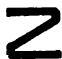
\includegraphics[keepaspectratio]{images/part002_1e1abfe7.jpg}}

The hypothesis that A is Noetherian cannot be omitted from the statement (Exercise 2).

DEFINITION 2. Let A be a ring. An A-algebra R (not necessarily commutative) is called integral over A if every element of R is integral over A. R is called finite over A if R is a finitely generated A-module.

It follows from Proposition 1 that every finite A-algebra is integral; if R is commutative and a finite A-algebra, R is obviously a finitely generated A-algebra; the converse is false.

Example (4) If M is a finitely generated A-module, the algebra \(\operatorname{End}_{\mathbf{A}}(\mathbf{M})\) of endomorphisms of M is integral over A by virtue of \((\mathrm{E}_{\mathrm{III}})\) ; in particular, for every integer n, the matrix algebra \(\mathbf{M}_{n}(\mathbf{A}) = \operatorname{End}_{\mathbf{A}}(\mathbf{A}^{n})\) is integral (and even finite) over A.

PROPOSITION 2. Let A, A' be two rings, R an A-algebra, R' an A'-algebra (not necessarily commutative) and \(f\colon\mathbf{A}\to\mathbf{A}'\) and \(g\colon\mathbf{R}\to\mathbf{R}'\) two ring homomorphisms such that the diagram

\pandocbounded{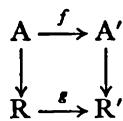
\includegraphics[keepaspectratio]{images/part002_4af46373.jpg}}

is commutative. If an element \(x \in R\) is integral over A, then \(g(x)\) is integral over \(A'\) . If \(x^{n} + a_{1}x^{n-1} + \cdots + a_{n} = 0\) where \(a_{i} \in A\) for \(1 \leqslant i \leqslant n\) , we deduce that

\[
(g (x)) ^ {n} + f \left(a _ {1}\right) (g (x)) ^ {n - 1} + \dots + f \left(a _ {n}\right) = 0.
\]

COROLLARY 1. Let A be a ring, B a (commutative) A-algebra and C a (not necessarily commutative) B-algebra. Then every element \(x \in \mathbf{C}\) which is integral over A is integral over B.

COROLLARY 2. Let K be a field, L an extension of K and x, \(x'\) two elements of L which are conjugate over K (Algebra, Chapter V, § 6, no. 2). If A is a subring of K and x is integral over A, \(x'\) is also integral over A.

There exists a K-isomorphism \(f\) of \(\mathbf{K}(x)\) onto \(\mathbf{K}(x')\) such that \(f(x) = x'\) and the elements of \(\mathbf{A}\) are invariant under \(f\) .

COROLLARY 3. Let A be a ring, B a (commutative) A-algebra and C a (not necessarily commutative) B-algebra. If C is integral over A, C is integral over B.

PROPOSITION 3. Let \((\mathbf{R}_i)_{1\leqslant i\leqslant n}\) be a finite family of (not necessarily commutative)

A-algebras and let \(\mathbf{R} = \prod_{i=1}^{n} \mathbf{R}_i\) be their product. For an element \(x = (x_i)_{1 \leq i \leq n}\) of \(\mathbf{R}\) to be integral over \(\mathbf{A}\) , it is necessary and sufficient that each of the \(x_i\) be integral over \(\mathbf{A}\) . For \(\mathbf{R}\) to be integral over \(\mathbf{A}\) , it is necessary and sufficient that each of the \(\mathbf{R}_i\) be integral over \(\mathbf{A}\) .

It is obviously sufficient to prove the first assertion. The condition is necessary by Proposition 2. Conversely, if each of the \(x_{i}\) is integral over \(A\) , the subalgebra \(A[x_{i}]\) of \(R_{i}\) is a finitely generated \(A\) -module and hence so is the subalgebra \(\prod_{i=1}^{n} \mathrm{A}[x_i]\) of R; as \(\mathrm{A}[x]\) is contained in this subalgebra, \(x\) is integral over A by Proposition 1.

PROPOSITION 4. Let A be a ring, R an A-algebra (not necessarily commutative) and \((x_{i})_{1\leq i\leq n}\) a finite family of elements of R which are pairwise permutable. If, for all \(i, x_{i}\) is integral over \(A[x_{1},\cdots,x_{i-1}]\) (and in particular if all the \(x_{i}\) are integral over A), then the subalgebra \(A[x_{1},\ldots,x_{n}]\) of R is a finitely generated A-module.

We argue by induction on \(n\) , the proposition being just \((\mathbf{E}_{\mathrm{II}})\) for \(n = 1\) . The induction hypothesis implies that \(B = A[x_{1}, \cdots, x_{n-1}]\) is a finitely generated A-module; as \(x_{n}\) is integral over B, \(B[x_{n}] = A[x_{1}, \cdots, x_{n}]\) is a finitely generated B-module and therefore also a finitely generated A-module (Algebra, Chapter II, § 1, no. 13, Proposition 25).

COROLLARY 1. Let A be a ring and R a (commutative) A-algebra. The set of elements of R integral over A is a subalgebra of R.

In fact, if x, y are two elements of R integral over A, it follows from Proposition 4 that A{[}x, y{]} is a finitely generated A-module; as it contains \(x + y\) and xy, the corollary follows from Proposition 1.

\pandocbounded{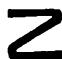
\includegraphics[keepaspectratio]{images/part002_90735efb.jpg}}

In a non-commutative algebra the sum and product of two integral elements over A are not necessarily integral over A (Exercise 4).

COROLLARY 2. Let A be a ring, R an A-algebra (not necessarily commutative) and E a set of elements of R which are pairwise permutable and integral over A. Then the sub-A-algebra B of R generated by E is integral over A.

Every element of B belongs to a sub-A-algebra of B generated by a finite subset of E.

Remark (3) It follows from Proposition 4 that every commutative A-algebra integral over A is the union of a right directed family of finite subalgebras over A.

PROPOSITION 5. Let A be a ring and A' and R two (commutative) A-algebras. If R is integral over A, \(R \otimes_{A} A'\) is integral over A'.

Consider any element \(x' = \sum_{i=1}^{n} x_i \otimes a_i'\) of \(\mathbf{R} \otimes_{\mathbf{A}} \mathbf{A}'\) , where the \(x_i\) belong to \(\mathbf{R}\) and the \(a_i'\) to \(\mathbf{A}'\) ; as \(x_i \otimes a_i' = (x_i \otimes 1)a_i'\) and the \(x_i \otimes 1\) are integral over \(\mathbf{A}'\) (Proposition 2), so is \(x\) .

COROLLARY. Let R be a ring and A, B, C subrings of R such that \(A \subset B\) . If B is integral over A, C{[}B{]} is integral over C{[}A{]}.

\(B \otimes_{A} C[A]\) is integral over \(C[A]\) by Proposition 5 and hence so is the canonical image \(C[B]\) of \(B \otimes_{A} C[A]\) in \(R\) (considered as an A-algebra) by Proposition 2.

PROPOSITION 6. Let A be a ring, B a (commutative) A-algebra and C a (not necessarily commutative) B-algebra. If B is integral over A and C is integral over B, then C is integral over A.

It is sufficient to verify that every \(x \in C\) is integral over A. By hypothesis there exists a monic polynomial \(X^{n} + b_{1}X^{n-1} + \cdots + b_{n}\) with coefficients in B with x as a root; then x is integral over \(B' = A[b_{1}, \ldots, b_{n}]\) and \(B'[x]\) is therefore a finitely generated \(B'\) -module. But as B is integral over A, \(B'\) is a finitely generated A-module (Proposition 4); we conclude that \(\mathbf{B}'[x]\) is also a finitely generated A-module (Algebra, Chapter II, §1, no. 13, Proposition 25) and therefore \(x\) is integral over \(\mathbf{A}\) .

COROLLARY. Let A be a ring and R, R' two (commutative) A-algebras integral over A. Then \(R \otimes_{A} R'\) is integral over A.

\(R \otimes_{A} R'\) is integral over \(R'\) (Proposition 5) and hence the conclusion follows from Proposition 6.

\subsection{The integral closure of a ring. Integrally closed domains}

DEFINITION 3. Let A be a ring and R a (commutative) A-algebra. The sub-A-algebra A' of R consisting of the elements of R integral over A (no. 1, Corollary 1 to Proposition 4) is called the integral closure of A in R. If A' is equal to the canonical image of A in R, A is called integrally closed in R.

\textbf{Remarks}\par

\begin{enumerate}
\def\labelenumi{(\arabic{enumi})}
\item
  If \(h: \mathbf{A} \to \mathbf{R}\) is the ring homomorphism defining the A-algebra structure on \(\mathbf{R}\) , the integral closure of \(\mathbf{A}\) in \(\mathbf{R}\) is also that of \(h(\mathbf{A})\) in \(\mathbf{R}\) . On the other hand, if \(\mathbf{R}'\) is a subalgebra of \(\mathbf{R}\) , the integral closure of \(\mathbf{A}\) in \(\mathbf{R}'\) is \(\mathbf{A}' \cap \mathbf{R}'\) .
\item
  If A is a field, the integral closure \(A'\) of A in R consists of the elements of R which are algebraic over A (no. 1, Example 1); generalizing the terminology used for field extensions (Algebra, Chapter V, §3, no. 3), \(A'\) is then also called the algebraic closure of the field A in the algebra R and A is called algebraically closed in R if \(A' = A\) .
\end{enumerate}

DEFINITION 4. If A is an integral domain, the integral closure of A in its field of fractions is called the integral closure of A. An integral domain is called integrally closed if it is equal to its integral closure.

\pandocbounded{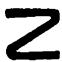
\includegraphics[keepaspectratio]{images/part002_6bc214f1.jpg}}

Note that an integrally closed domain is not necessarily closed in any ring containing it, as the example of a field which is not algebraically closed shows.

PROPOSITION 7. Let A be a ring and R an A-algebra. The integral closure A' of A in R is a subring integrally closed in R.

The integral closure of A' in R is integral over A by no. 1, Proposition 6; it is therefore equal to A'.

COROLLARY. The integral closure of an integral domain A is an integrally closed domain.

Let K be the field of fractions of A and B the integral closure of A. Clearly

K is the field of fractions of B and it is sufficient to apply Proposition 7 to R = K.

PROPOSITION 8. Let R be a ring, \((\mathbf{B}_{\lambda})_{\lambda \in \mathbf{L}}\) a family of subrings of R and for each \(\lambda \in L\) let \(A_{\lambda}\) be a subring of \(B_{\lambda}\) . If each \(A_{\lambda}\) is integrally closed in \(B_{\lambda}\) , then \(A = \bigcap_{\lambda \in L} A_{\lambda}\) is integrally closed in \(B = \bigcap_{\lambda \in L} B_{\lambda}\) .

This follows immediately from Definition 3 and no. 1, Corollary 1 to Proposition 2.

COROLLARY. Every intersection of a non-empty family of integrally closed subdomains of an integral domain A is an integrally closed domain.

It is sufficient to apply Proposition 8 taking R and the \(B_{\lambda}\) equal to the field of fractions K of A and noting that a subring of K integrally closed in K is a fortiori an integrally closed domain since its field of fractions is contained in K.

PROPOSITION 9. Let A be a ring, \((\mathbf{R}_i)_{1 \leqslant i \leqslant n}\) a finite family of A-algebras and \(\mathbf{A}_i'\) the integral closure of A in \(\mathbf{R}_i\) ( \(1 \leqslant i \leqslant n\) ). Then the integral closure of A in \(\mathbf{R} = \prod_{i=1}^{n} \mathbf{R}_i\) is equal to \(\prod_{i=1}^{n} \mathbf{A}_i'\) .

This is an immediate consequence of no. 1, Proposition 3.

COROLLARY 1. Let A be a reduced Noetherian ring, \(\mathfrak{p}_i\) ( \(1 \leqslant i \leqslant n\) ) its distinct minimal prime ideals, \(\mathbf{K}_i\) the field of fractions of the integral domain \(\mathbf{A} / \mathfrak{p}_i\) (canonically isomorphic to the local ring \(\mathbf{A}_{\mathfrak{p}_i}\) (Chapter IV, §2, no. 5, Proposition 10)) and \(\mathbf{A}_i'\) the integral closure of A in \(\mathbf{K}_i\) ( \(1 \leqslant i \leqslant n\) ). Then the canonical isomorphism of the total ring of fractions B of A onto \(\prod_{i=1}^{n} \mathbf{K}_i\) (loc. cit.) maps the integral closure of A in B onto the product ring \(\prod_{i=1}^{n} \mathbf{A}_i'\) .

COROLLARY 2. For a reduced Noetherian ring to be integrally closed in its ring of fractions it is necessary and sufficient that it be a direct composition of integrally closed (Noetherian) domains.

\subsection{Examples of integrally closed domains}

PROPOSITION 10. Every principal ideal domain is integrally closed.\par

Let A be a principal ideal domain, K its field of fractions and x an element of K. There exist two relatively prime elements a, b of A such that \(x = ab^{-1}\) (Algebra, Chapter VII, §1, no. 2, Proposition 1 and Chapter VI, §1, no. 11, Proposition 9 (DIV)). If x is integral over A, it is a root of a polynomial

\(X^{n} + c_{1}X^{n-1} + \cdots + c_{n}\) of A{[}X{]}. Then \(a^{n} = b(-c_{1}a^{n-1} - \cdots - c_{n}b^{n-1})\) , which proves that \(b\) divides \(a^{n}\) . Since \(a\) and \(b\) are relatively prime, this implies that \(b\) is invertible in A (Algebra, Chapter VI, § 1, no. 12, Corollary 1 to Proposition 11 (DIV)); hence \(x \in A\) .

LEMMA 2. Let R be a ring and P a monic polynomial in R{[}X{]}. There exists a ring R' containing R such that in the polynomial ring R'{[}X{]} the polynomial P is a product of monic polynomials of degree 1.

We proceed by induction on the degree \(n\) of \(\mathbf{P}\) , the lemma being obvious for \(n = 0\) and \(n = 1\) . Suppose therefore that \(n > 1\) . Let \(\mathfrak{a}\) be the ideal of \(\mathbb{R}[\mathbf{X}]\) generated by \(\mathbf{P}\) and let \(f\) be the canonical homomorphism of \(\mathbb{R}[\mathbf{X}]\) onto \(\mathbf{B} = \mathbb{R}[\mathbf{X}] / \mathfrak{a}\) . Since \(\mathbf{P}\) is monic, for every polynomial \(\mathbf{Q} \in \mathbb{R}[\mathbf{X}]\) , \(\deg(\mathrm{PQ}) = \deg(\mathrm{P}) + \deg(\mathrm{Q})\) , whence \(\mathfrak{a} \cap \mathbb{R} = 0\) ; the restriction of \(f\) to \(\mathbb{R}\) is therefore injective. Identifying \(\mathbb{R}\) with the subring \(f(\mathbb{R})\) of \(\mathbb{B}\) by means of \(f\) and writing \(b = f(\mathbf{X})\) , we see that \(b\) is a root of \(\mathbf{P}\) in \(\mathbb{B}\) , \(\mathbf{P}\) being considered as a polynomial in \(\mathbb{B}[\mathbf{X}]\) . Then there exists a monic polynomial \(\mathbf{Q}\) in \(\mathbb{B}[\mathbf{X}]\) of degree \(n - 1\) such that \(\mathrm{P}(\mathbf{X}) = (\mathbf{X} - b)\mathrm{Q}(\mathbf{X})\) (Algebra, Chapter IV, § 1, no. 4, Proposition 5). By the induction hypothesis there exists a ring \(\mathbb{R}' \supseteq \mathbb{B}\) such that in \(\mathbb{R}'[\mathbf{X}]\) the polynomial \(\mathbf{Q}\) is a product of monic polynomials of degree 1; clearly in \(\mathbb{R}'[\mathbf{X}]\) \(\mathbf{P}\) is then a product of monic polynomials of degree 1.

PROPOSITION 11. Let A be a ring, R an A-algebra and P and Q monic polynomials in R{[}X{]}. If the coefficients of PQ are integral over A, the coefficients of P and Q are integral over A.

By a double application of Lemma 2, we see that there exists a ring \(\mathbf{R}'\) containing \(\mathbf{R}\) and families of elements \((a_i)_{1 \leqslant i \leqslant m}, (b_j)_{1 \leqslant j \leqslant n}\) of \(\mathbf{R}'\) such that in \(\mathbf{R}'[\mathbf{X}]\) \(\mathrm{P}(\mathbf{X}) = \prod_{i=1}^{m} (\mathbf{X} - a_i)\) , \(\mathbf{Q}(\mathbf{X}) = \prod_{j=1}^{n} (\mathbf{X} - b_j)\) ; the coefficients of \(\mathbf{PQ}\) belong to the integral closure \(\mathbf{A}'\) of \(\mathbf{A}\) in \(\mathbf{R}'\) and hence (no. 2, Proposition 7) the elements \(a_i\) ( \(1 \leqslant i \leqslant m\) ) and \(b_j\) ( \(1 \leqslant j \leqslant n\) ) belong to \(\mathbf{A}'\) . It follows that the coefficients of \(\mathbf{P}\) and \(\mathbf{Q}\) are integral over \(\mathbf{A}\) (no. 1, Corollary 1 to Proposition 4).

Let A be an integral domain, K its field of fractions and \(K'\) a K-algebra (not necessarily commutative). Given an element \(x \in K'\) algebraic over K, the polynomials \(P \in K[X]\) such that \(P(x) = 0\) form an ideal \(a \neq 0\) of \(K[X]\) , necessarily principal (Algebra, Chapter IV, §1, no. 5, Proposition 7). There exists a unique monic polynomial which generates a; generalizing the terminology introduced in Algebra, Chapter V, §3, no. 1, Definition 3, this monic polynomial will be called the minimal polynomial of x over K.

COROLLARY. Let A be an integral domain, K its field of fractions and x an element of a K-algebra \(K'\) (not necessarily commutative). If x is integral over A, the coefficients of the minimal polynomial P of x over K are integral over A (and they therefore belong to A if A is integrally closed).

There exists by hypothesis (no. 1, Theorem 1) a monic polynomial \(Q \in A[X]\) such that \(Q(x) = 0\) . As P divides Q in K{[}X{]}, it follows from Proposition 11 that the coefficients of P are integral over A.

Let A be a ring and R a (commutative) A-algebra; the homomorphism \(\phi: A \rightarrow R\) defining the A-algebra structure on R can be extended uniquely to a homomorphism \(A[X] \rightarrow R[X]\) of polynomial rings over A and R, leaving X invariant and hence \(R[X]\) is given a canonical A{[}X{]}-algebra structure.

PROPOSITION 12. Let A be a ring, R an A-algebra and P a polynomial in \(R[X_{1},\ldots,X_{n}]\) . For P to be integral over \(A[X_{1},\ldots,X_{n}]\) , it is necessary and sufficient that the coefficients of P be integral over A.

By considering the polynomials of \(R[X_{1},\ldots,X_{n}]\) as polynomials in \(X_{n}\) with coefficients in \(R[X_{1},\ldots,X_{n-1}]\) , we see immediately that it is reduced to proving the proposition for n=1. Then let P be a polynomial in \(R[X]\) ; it follows immediately from no. 1, Proposition 5 that, if the coefficients of P are in the integral closure B of A in R, the element P, which belongs to \(B[X]=B\otimes_{A}A[X]\) , is integral over A{[}X{]}. Conversely, suppose that P is integral over A{[}X{]} and let

\[
\mathrm{Q} (\mathrm{Y}) = \mathrm{Y} ^ {m} + \mathrm{F} _ {1} \mathrm{Y} ^ {m - 1} + \dots + \mathrm{F} _ {m}
\]

be a monic polynomial with coefficients \(F_{i} \in A[X]\) with P as a root. Let r be an integer strictly greater than all the degrees of the polynomials P and \(F_{i}\) ( \(1 \leqslant i \leqslant m\) ) and let us write

\[
\mathrm{P} _ {1} (\mathrm{X}) = \mathrm{P} (\mathrm{X}) - \mathrm{X} ^ {r}.
\]

Then \(\mathbf{P}_1\) is a root of the polynomial

\[
\mathrm{Q} _ {1} (\mathrm{Y}) = \mathrm{Q} (\mathrm{Y} + \mathrm{X} ^ {r}) = \mathrm{Y} ^ {m} + \mathrm{G} _ {1} \mathrm{Y} ^ {m - 1} + \dots + \mathrm{G} _ {m}
\]

with coefficients in A{[}X{]}; we may therefore write

\[
- \mathrm{P} _ {1} (\mathrm{P} _ {1} ^ {m - 1} + \mathrm{G} _ {1} \mathrm{P} _ {1} ^ {m - 2} + \dots + \mathrm{G} _ {m - 1}) = \mathrm{G} _ {m}.\tag{1}
\]

Now the choice of \(r\) implies that \(-\mathbf{P}_1\) is a monic polynomial of \(\mathbb{R}[\mathbf{X}]\) and so is \(\mathbf{G}_m(\mathbf{X}) = \mathbf{Q}(\mathbf{X}^r)\) , the degrees of the polynomials \(\mathrm{F}_k(\mathbf{X})\mathbf{X}^{r(m - k)}\) being all \(< rm\) for \(k \geqslant 1\) . We conclude first of all that the polynomial

\[
\mathrm{P} _ {1} ^ {m - 1} + \mathrm{G} _ {1} \mathrm{P} _ {1} ^ {m - 2} + \dots + \mathrm{G} _ {m - 1}
\]

of R{[}X{]} is also monic; moreover, as the coefficients of \(G_{m}\) belong to A, Proposition 11 shows that \(P_{1}\) has coefficients integral over A and the coefficients of P are therefore certainly integral over A.

PROPOSITION 13. Let A be a ring, R an A-algebra and A' the integral closure of A in R. Then the integral closure of A{[}X₁, \ldots, Xₙ{]} in R{[}X₁, \ldots, Xₙ{]} is equal to A'{[}X₁, \ldots, Xₙ{]}.

This follows from Proposition 12 and Definition 3 of no. 2.

COROLLARY 1. Let A be an integral domain and A' its integral closure. Then the integral closure of the polynomial ring A{[}X₁, \ldots, Xₙ{]} is A'{[}X₁, \ldots, Xₙ{]}.

Arguing by induction on n, the problem is immediately reduced to the case n = 1. Let K be the field of fractions of A, which is also that of A'; if an element P of the field of fractions K(X) of A{[}X{]} is integral over A{[}X{]}, it belongs to the polynomial ring K{[}X{]}, for the latter is a principal ideal domain (Algebra, Chapter IV, § 1, no. 5, Proposition 7) and hence integrally closed (Proposition 10); the corollary then follows from Proposition 13 applied to R = K.

COROLLARY 2. Let A be an integral domain. For the polynomial ring A{[}X \(_{1}\) , \ldots, X \(_{n}\) {]} to be integrally closed, it is necessary and sufficient that A be integrally closed.

COROLLARY 3. If K is a field, every polynomial algebra \(\mathbf{K}[\mathbf{X}_1,\ldots ,\mathbf{X}_n]\) is an integrally closed domain.

\subsection{Completely integrally closed domains}

DEFINITION 5. An integral domain A is called completely integrally closed if the following condition is satisfied: every element x of the field of fractions K of A such that all the powers \(x^{n}\) ( \(n \geqslant 0\) ) are contained in a finitely generated sub-A-module of K, belongs to A.

Note that the hypothesis that the \(x^n\) are contained in a finitely generated sub-A-module of K can also be expressed by saying that there exists a non-zero element \(d \in \mathbf{A}\) such that \(dx^n \in \mathbf{A}\) for all \(n \geqslant 0\) ; for the latter condition means that \(x^n \in \mathrm{Ad}^{-1}\) ; and conversely, if \((b_i)_{1 \leqslant i \leqslant m}\) is a finite sequence of elements of K, there exists \(d \in \mathbf{A}\) such that \(db_i \in \mathbf{A}\) for \(1 \leqslant i \leqslant m\) , whence \(d\mathbf{M} \subset \mathbf{A}\) for the sub-A-module M of K generated by the \(b_i\) .

Clearly a completely integrally closed domain is integrally closed; conversely, the Corollary to Proposition 1 of no. 1 shows that an integrally closed Noetherian domain is completely integrally closed. * On the other hand, the ring of a valuation of height ≥ 2 (Chapter VI, § 4, no. 4) is integrally closed but not completely integrally closed. * If (A\_t) is a family of completely integrally closed domains with the same field of fractions K, A = ∩\_t A\_t is completely integrally closed. For if x ∈ K is such that for some non-zero d in A, \(dx^n\) belongs to A for all n \textgreater{} 0, the hypothesis implies that x ∈ A\_t for all t and hence x ∈ A.

PROPOSITION 14. Let A be a completely integrally closed domain. Then every polynomial ring \(\mathbf{A}[\mathbf{X}_1,\ldots ,\mathbf{X}_n]\) (resp. every ring of formal power series \(\mathbf{A}[[\mathbf{X}_1,\dots ,\mathbf{X}_n]]\) ) is completely integrally closed.

By induction on \(n\) , it is sufficient to prove that A{[}X{]} (resp. A{[}{[}X{]}{]}) is completely integrally closed. Then let P be an element of the field of fractions of A{[}X{]} (resp. A{[}{[}X{]}{]}) and suppose that there exists a non-zero element Q ∈ A{[}X{]} (resp. Q ∈ A{[}{[}X{]}{]}) such that QP \(^{m}\) ∈ A{[}X{]} (resp. QP \(^{m}\) ∈ A{[}{[}X{]}{]}) for every integer m ≥ 0. If K is the field of fractions of A, A{[}X{]} (resp. A{[}{[}X{]}{]}) is a subring of K{[}X{]} (resp. K{[}{[}X{]}{]}) and K{[}X{]} (resp. K{[}{[}X{]}{]}) is a principal ideal domain (Algebra, Chapter VII, § 1, no. 1) and hence integrally closed (no. 4, Proposition 10) and Noetherian (Algebra, Chapter VIII, § 2, no. 3) and therefore completely integrally closed; then we have already seen that \(\mathbf{P} \in \mathbf{K}[\mathbf{X}]\) (resp. \(\mathbf{P} \in \mathbf{K}[[\mathbf{X}]]\) ). Let \(\mathbf{P} = \sum_{k=0}^{\infty} a_k \mathbf{X}^k\) ( \(a_k \in \mathbf{K}\) ) and \(\mathbf{Q} = \sum_{k=0}^{\infty} b_k \mathbf{X}^k\) ( \(b_k \in \mathbf{A}\) ) and we argue by reductio ad absurdum by supposing that the \(a_k\) do not all belong to \(\mathbf{A}\) ; then there is a least index \(i\) such that \(a_i \notin \mathbf{A}\) ; if we write

\(P_{1}=\sum_{k=0}a_{k}X^{k}\in A[X]\) , it follows immediately from the hypothesis that also \(Q(P-P_{1})^{m}\in A[X]\) (resp. \(Q(P-P_{1})^{m}\in A[[X]]\) ) for all \(m\geqslant0\) . Let j be the least integer such that \(b_{j}\neq0\) ; clearly in \(Q(P-P_{1})^{m}\) the term of least degree with a coefficient \(\neq0\) is \(b_{j}a_{i}^{m}X^{j+m^{i}}\) and hence \(b_{j}a_{i}^{m}\in A\) for all \(m\geqslant0\) ; but as A is completely integrally closed this implies \(a_{i}\in A\) , contrary to the hypothesis.

PROPOSITION 15. Let A be a filtered ring whose filtration is exhaustive and such that every principal ideal of A is closed under the topology defined by the filtration. If the associated graded ring gr(A) (Chapter III, §2, no. 3) is a completely integrally closed domain, then A is a completely integrally closed domain.

Let \((\mathbf{A}_n)_{n\in \mathbf{Z}}\) be the filtration defined on \(\mathbf{A}\) ; as \(\bigcap_{n\in \mathbf{Z}}\mathbf{A}_n\) is the closure of the ideal (0) (Chapter III, § 2, no. 5), the hypothesis implies first that the filtration \((\mathbf{A}_n)\) is separated and, as \(\operatorname{gr}(\mathbf{A})\) is an integral domain, so then is \(\mathbf{A}\) (Chapter III, § 2, no. 3, Corollary to Proposition 1). Let \(x = b / a\) be an element of the field of fractions \(\mathbf{K}\) of \(\mathbf{A}\) ( \(a\in \mathbf{A}, b\in \mathbf{A}\) ) for which there exists an element \(d\neq 0\) of \(\mathbf{A}\) such that \(dx^n\in \mathbf{A}\) for all \(n\geqslant 0\) . We must prove that \(b\in \mathbf{A}a\) and, as by hypothesis the ideal \(\mathbf{A}a\) is closed, it is sufficient to show that, for all \(n\in \mathbf{Z}, b\in \mathbf{A}a + \mathbf{A}_n\) . As the filtration of \(\mathbf{A}\) is exhaustive, there exists an integer \(q\in \mathbf{Z}\) such that \(b\in \mathbf{A}a + \mathbf{A}_q\) . It will therefore suffice to prove that the relation \(b\in \mathbf{A}a + \mathbf{A}_m\) implies \(b\in \mathbf{A}a + \mathbf{A}_{m + 1}\) .

Suppose then that \(b = ay + z\) where \(y \in \mathbf{A}\) , \(z \in \mathbf{A}_m\) . Then by hypothesis \(dx^n \in \mathbf{A}\) for all \(n \geqslant 0\) , whence we obtain immediately \(d(x - y)^n \in \mathbf{A}\) for all \(n \geqslant 0\) ; in other words, \(dz^n = a^n t_n\) where \(t_n \in \mathbf{A}\) for all \(n \geqslant 0\) . We can obviously limit our attention to the case where \(z \neq 0\) . Let \(v\) denote the order function on \(\mathbf{A}\) (Chapter III, §1, no. 2) and let us write \(v(d) = n_1\) , \(v(z) = n_2 \geqslant m\) , \(v(a) = n_3\) ; let \(d', z', a'\) be the respective images of \(d, z, a\) in \(\mathbf{A}_{n_1}/\mathbf{A}_{n_1+1}\) , \(\mathbf{A}_{n_2}/\mathbf{A}_{n_2+1}\) , \(\mathbf{A}_{n_3}/\mathbf{A}_{n_3+1}\) . For all \(n \geqslant 0\) , \(v(dz^n) = n_1 + nn_2\) (Chapter III, §2, no. 3, Proposition 1) and hence the canonical image in \(\mathrm{gr}(\mathbf{A})\) of \(dz^n\) is \(d'z'^n\) ; similarly it is seen that the canonical image in \(\mathrm{gr}(\mathbf{A})\) of \(a^n t_n\) is of the form \(a'^n t_n'\) where \(t_n' \in \mathrm{gr}(\mathbf{A})\) and, as \(a' \neq 0\) we deduce that, for all \(n \geqslant 0\) , \(d'(z'/a')^n \in \mathrm{gr}(\mathbf{A})\) . The hypothesis that \(\mathrm{gr}(\mathbf{A})\) is completely integrally closed therefore implies the existence of an \(s' \in \mathrm{gr}(\mathbf{A})\) such that \(z' = a's'\) ; decomposing \(s'\) into a sum of homogeneous elements, it is further seen (since \(z'\) and \(a'\) are homogeneous) that \(s'\) may be assumed to be homogeneous, that is the image of an element \(s \in \mathbf{A}\) ; then \(v(as) = v(z) = n_2\) and \(z \equiv as (\mathrm{mod. A_{n_2+1}})\) ; as \(n_2 \geqslant m\) , a fortiori \(z \equiv as (\mathrm{mod. A_{m+1}})\) , hence \(b \equiv a(y + s) (\mathrm{mod. A_{m+1}})\) .
